\chapter{A new gamification framework and its implementation: the UMLegend tool}

\graphicspath{{Chapter4/}}

The findings described in the previous chapter highlighted the positive impact gamification can have on student performance, albeit with relevant limitations such as a rigid evaluation engine, which led to frustration and unfavorable reception of some game mechanics, and the inability to properly evaluate long-term mechanics defined in the original prototype such as leaderboards and experience points. A new research activity started after the empirical experiment aimed at addressing the existing limitations and generalize the tool to be suitable for other modeling topics: the end goal was to design a new gamified framework starting from what was implemented in BIPMIN to support both exercise activities and long-term use; the new framework would then be used to lead the development of tools that could support different modeling notations, with the goal of merging all tools in a complete educational platform for software modeling.

This chapter describes the design of the new framework and its application in the development of a tool named UMLegend, a web platform developed from spring 2023 for gamifying UML class diagram modeling; furthermore, the chapter also discusses the empirical experiment that was performed to evaluate UMLegend's impact on student performance, as well as how a tool implemented according to the new framework would be perceived compared to the original BIPMIN implementation of certain game mechanics. The UMLegend tool was first presented in \cite{cagnazzo_2023_umlegend}, while the empirical experiment and its results were described in both \cite{garaccione_2024_sqj} and \cite{garaccione_2026_gamification}.


\section{Background and Motivation}
\label{sec:back4}

One of the main research goals, following the empirical experiment, was to develop a generalized gamified platform for software modeling disciplines; thus, other relevant notations were considered for analysis as part of the development effort and, among them, the Unified Modeling Language (UML) was selected as the set of target notations. UML offers many diagram types, which can be used in different steps of the software engineering process such as requirements definition, system and architecture design, use case specification, and activity sequencing.

Class diagrams were selected as the main type of diagram acting as focus of the research activity, due to their diffusion as an effective instrument for requirements engineering and object-oriented development; a general description of the notation and its key components was introduced back in Section \ref{sec:back_mde}. 

%Even if Class Diagram modeling is typically taught as a part of Software Engineering programs in Computer Science curricula, the topic is often seen as secondary with respect to software design and development. The pedagogy of conceptual modeling education has been extensively studied in related literature, highlighting a diffuse tendency among students to repeat some specific categories of errors, and the necessity of a significant amount of practice to acquire sufficient proficiency \cite{bogdanova2019towards}. Several studies in the literature have analyzed methodologies and techniques to enhance the motivation and engagement of students. Tools to automatically generate exercises and variations have been proposed, however the generation of new exercises - albeit indeed beneficial for learning - might not be helpful if the activities to perform are perceived as monotonous and cumbersome. To intrinsically motivate students in performed activities, Gamification (i.e., the application of game design elements in non-game contexts \cite{gamification}) has affirmed and has been deeply studied in the recent literature as a means capable of having positive impacts on students' learning experience and perception of learning activities \cite{marin_bookchapter}.

As discussed back in Section \ref{sec:back_gamif_mde}, examples of gamification and serious games being used to support UML class diagram education are more common compared to BPMN, and this required the  identification of gaps in the literature before starting the design of the new framework. For this purpose, a mapping review was performed in spring 2023 to identify relevant sources; the mapping was performed as a quasi-systematic literature research using the Google Scholar library, using \textit{gamif* class diagram} as the search string. The mapping analysis was executed according to the guidelines by Garousi et al. \cite{garousi2019guidelines} for conducting literature reviews: exclusion criteria were defined systematically, the goal was stated as \textit{identifying sources in the literature describing gamified tools and serious games for UML class diagram education}, and the stopping criterion adopted was an effort-bounded one.

All papers that resulted with the string were collected and their title, abstract, and keywords read to determine whether they could be considered a valid source: papers were excluded if they did not explicitly cover class diagrams, if they did not apply gamification or were not describing a serious game, if they were written in a non-English language, and if they were not white literature papers but rather theses, preprints, or non-peer reviewed papers. The search process was performed until a full page of Google Scholar results contained only papers that satisfied at least one of the exclusion criteria mentioned above, resulting in 10 consecutive rejected papers.

The search analyzed a total of 80 papers, 16 of which described either a gamified tool or a serious game, with one preprint, resulting in a total of 15 sources; this set of papers was then extended with 7 additional papers that were found separately from the search but were considered relevant for the literature analysis. The tools and serious games identified by the mapping are described in Section \ref{sec:back_gamif_mde}, together with the result of the analysis conducted on them.

%The full list of papers, including the excluded papers and the result of the mapping, is available online.\footnote{\url{https://doi.org/10.6084/m9.figshare.25968082.v2}}

The literature analysis showed that existing gamified solutions for class diagram education are not common, and the existing ones offer static exercise-solving capabilities, where students can only choose alternatives out of a predefined set of options, reinforcing the need for a solution similar to BIPMIN that could let students freely draw their intended solutions. Furthermore, most solutions highlight the importance of mechanics such as level progression, unlockable rewards, leaderboards, and feedback. 


Furthermore, another limitation that emerged after the experiment related to the evaluation engine, whose implementation was too strict and reliant on a single reference solution with multiple elements needing to be correct at the same time to have a valid solution; with the decision to explore gamification of UML class diagrams as the next research step, an exploration of the existing research literature was performed in parallel to the gamification-focused analysis to define development decisions that would guide the design of the new tool. 
 
Following the results of the experiment and the literature analysis, it became clear that a new tool for UML diagrams would have to be completely reorganized in terms of how the game mechanics interact with the automated evaluation engine: the fact that both experiments were conducted over a single session meant that mechanics focused on long-term usage were less appreciated; the empirical experiment tried to mitigate this dependency by selecting only mechanics that were intended to work in the context of a single exercise, resulting in a single section of the interface containing all game elements, possibly making it harder to distinguish them and reducing their appreciation. Participants in the preliminary evaluation also mentioned that they would have preferred to experience mechanics such as avatars and leaderboards over longer periods of use, supporting the need to distinguish mechanics that depend on a single exercise (\textit{exercise-specific)} and those that impact the students' experience (\textit{long-term)} over time. 

Once the two categories of game mechanics had been identified, the subsequent design step was to assess which of the mechanics would have to be kept, considering the set of mechanics implemented in the original prototype version together with the ones selected for the empirical study. For what concerns long-term mechanics, avatars and leaderboards were selected, due to their appreciation in the preliminary study, with levels and experience points also being kept and considered as such, since most works in the literature considered them to be an effective mechanic.

For what concerns the exercise-specific mechanics, instead, the empirical experiment showed that the most appreciated mechanics were those that students could use to understand the correct elements of their solution and how close they were to completion (diagram feedback and the progress indicator): it was thus decided to redesign the mechanics connected to the modeling interface itself so that they could provide additional feedback by depending directly on the results of an automated evaluation.



\section{Tool Description and Features}

The design choices made following the experiment and the literature analysis guided the development of UMLegend, which was implemented starting from a Master Thesis as a web application intended for long-term modeling use. As a consequence, the tool had to be implemented in a way that would allow students to perform multiple exercises and see their overall progression, and support for teachers would also be needed as well for features such as creating new exercises with their intended solution, creating student accounts, or viewing statistics related to the students' performance; creation features were not implemented in the BIPMIN version used for the study, since exercises, solutions, and accounts were hard-coded in the tool, which made the implementation unfeasible if the end goal was long-term usage. 

This led to the development of separate client interfaces depending on the type of user account: Teacher accounts had access to a dashboard where they could create exercises by specifying description, difficulty level, experience reward, and reference solution through a form where expected classes, attributes, and associations could be expressed; student account creation was also supported, together with a dedicated section where saved exercise data could be seen and downloaded with the saved diagrams.

Student accounts, instead, could see the list of available exercises, a personal page for their profile, and a modeling page for each exercise. Modeling functionalities were achieved through the open-source Apollon library \cite{krusche2020interactive}, which offers an easy to use modeling canvas through a drag-and-drop functionality, with UML constructs being shown on the right side of the canvas and easy editing and connecting of elements, as can be seen in Figure \ref{fig:modeler}; the library also supports export capabilities in SVG or PDF format, and expresses a diagram's source code using the JSON format for easy readability.

\begin{figure*}[ht]
    \centering
    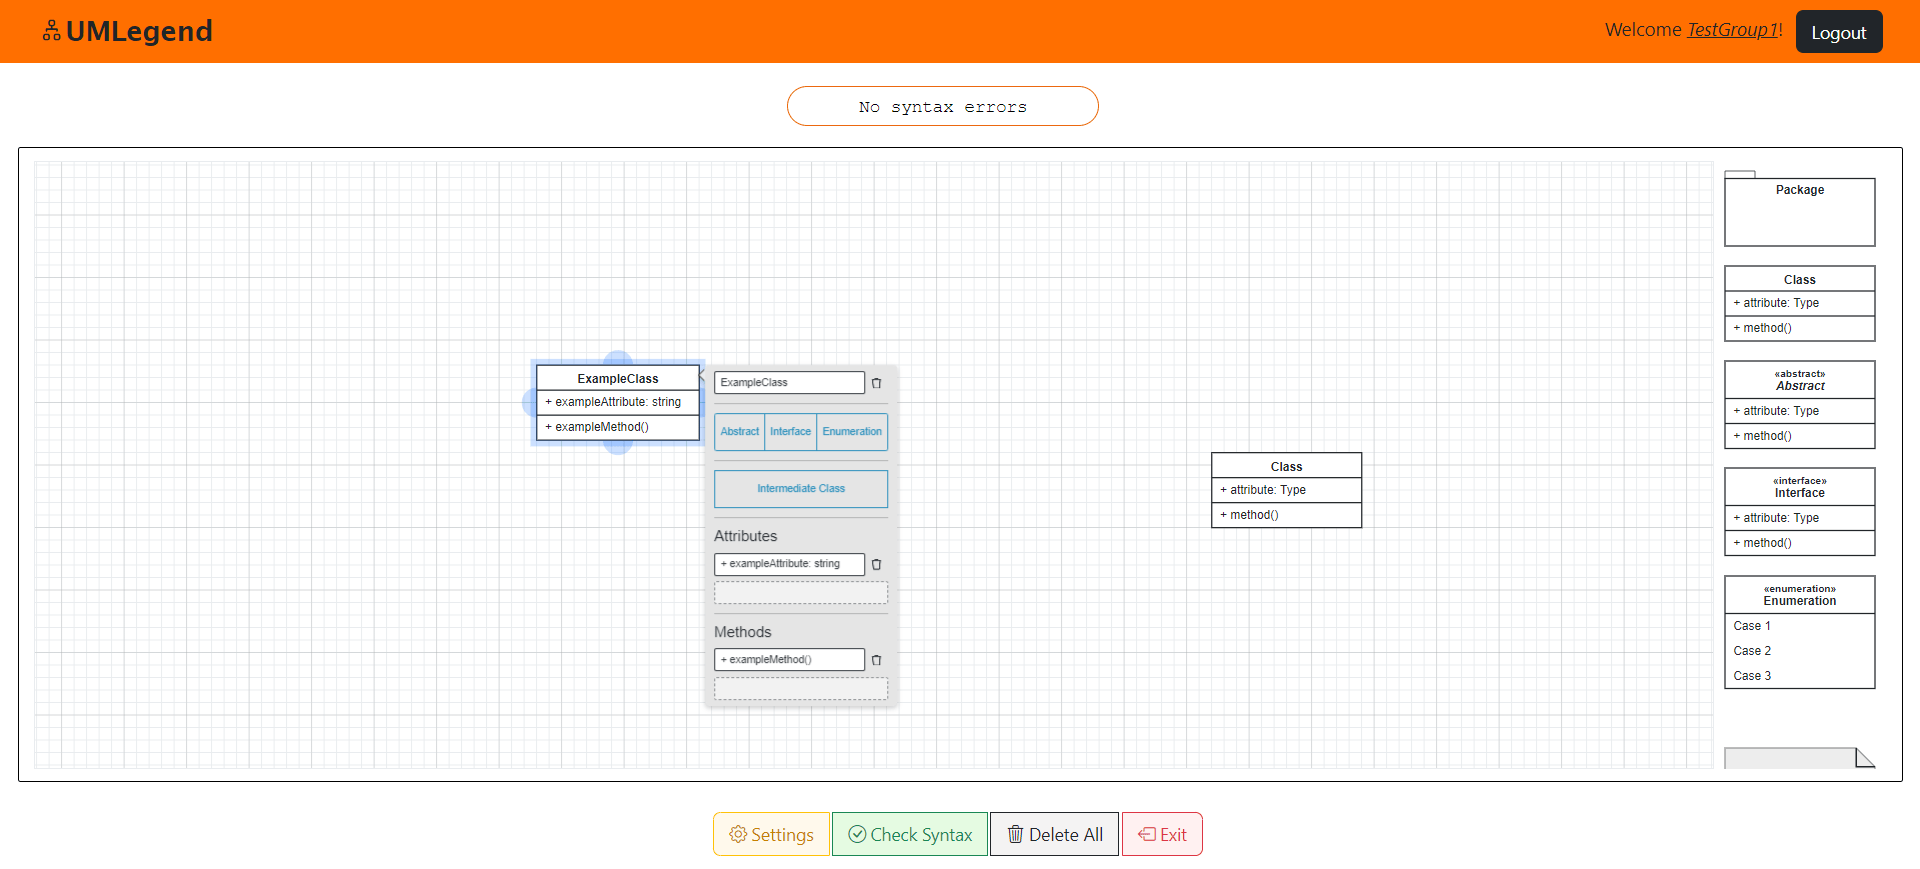
\includegraphics[width=\linewidth]{Template_Latex_ScuDo_Tesi/Chapter4/modeler.png}
    \caption{Base modeler of the UMLegend tool}
    \label{fig:modeler}
\end{figure*}

\begin{comment}

A visual representation of how the tool is structured can be seen in Figure \ref{fig_deploy}, the web server is a single entity, while the two clients can be accessed from any device, meaning that students can resume their work thanks to their account storing the entire history of their exercises.

\begin{figure}
    \centering
    \includegraphics[width=\columnwidth]{Fig2.eps}
    \caption{Component diagram representing the UMLegend tool}
    \label{fig_deploy}
\end{figure}
    
\end{comment}

\subsection{Gamified Mechanics}\label{sec:mechanics}

As mentioned at the end of Section \ref{sec:back4}, the game mechanics were redesigned by dividing them into two categories: exercise-specific mechanics that depend on a student's action and impact how they perceive the modeling assignment, and long-term mechanics that define a user's progression and depend on the performance over multiple exercises. 

Three long-term mechanics were selected for development inside UMLegend: levels and experience points, avatar customization, and leaderboards. These mechanics were selected since they represent a student's growing skill in modeling over time and help maintain engagement beyond usage for a single exercise.

\textbf{Levels and Experience points} were used to implement the primary progression system of students, who gain experience by completing an exercise when they reach a sufficient completeness score in an exercise, with the possibility to obtain additional bonuses in case of good performance such as attempting an exercise with a higher level, requiring a low number of checks to complete an exercise, or reaching an higher score than the minimum completion threshold. This mechanic was already present in the original prototype, where it was paired with leaderboards, and it was decided to implement it as a long-term mechanic to have a clear indicator of skill growth, in line with existing studies that used it in a similar way.

\textbf{Avatars} were one of the most appreciated mechanics in terms of enjoyment when the preliminary study was conducted, warranting their inclusion in the new tool; they showed, however, a comparatively lower score in terms of motivational impact, perhaps due to the fact that all available avatars were obtainable from the beginning, with no additional unlockable avatars being provided as a reward for good performance. For this reason, avatars were tied to level progression, making sure that leveling up served a purpose beyond showing the students' growing skill level; furthermore, the implementation itself was reworked: rather than a set of static avatars, the UMLegend tool used an external library to render human avatars with a wide range of customizable options such as clothing, hair, facial hair, accessories, and coloring, with most options being unlocked by leveling up. Avatar customization was added to UMLegend so that students could personalize their experience and express their individuality, starting from a randomly generated avatar whose look can be refined, and with rarer avatar props being obtainable only at higher level to introduce a degree of challenge.

\textbf{Leaderboards} act as the last long-term mechanic, since they were another underappreciated mechanic in the preliminary study but with potential for long term use. The addition of a customizable avatar system also tied better with the concept of leaderboards, since students could see the look of their peers and feel motivated to compete more by seeing what props could be obtained at different levels. Two leaderboard types were defined as a way for students to see their ranking: one global leaderboard that would order students according to their level first and by experience points after, and a second type of leaderboard, in place for each exercise and using the correctness score as the ranking.


Exercise-specific mechanics, instead, were selected as a way to enhance the actual modeling activity, with guiding students toward learning correct modeling practices as the main focus behind their selection and design. Certain of these mechanics are new ones, compared to both the preliminary prototype and the empirical experiment, while others have been retained and changed according to the experiment's result. These mechanics interact directly with the student, since they depend on the results of an automated evaluation, and modify both the tool interface and the modeling canvas itself as a consequence of good or bad performance; exercise-specific mechanics are avatar feedback, indicators, error lists, diagram feedback, and the in-exercise leaderboard. 

\textbf{Avatar Feedback} is a new mechanic that was selected as a consequence of the reworked avatar system: the intention behind using human avatars was to have a stand-in for the student themselves, which they could use to see themselves in the leaderboard, and the association between students and their avatars was taken one step further by placing the avatar directly in the exercise page where they could react to the modeling choices and the corresponding evaluation. A student's avatar changes its expression the more errors are made and the obtainable experience is reduced, starting from a smiling expression and becoming sadder over time the more this value falls; this implementation adds a negative motivator to discourage students from performing multiple evaluations with no significant difference, guiding them toward making careful and calculated changes. An example of how the avatar looks like when the obtainable experience points are low because of multiple mistakes is shown in Figure \ref{fig_tool}(1).

\textbf{Indicators} were already implemented in the prototype version, and an indicator showing the completeness percentage was well received in the empirical experiment, confirming the potential effectiveness of this mechanic. The revised gamification framework, and the subsequent UMLegend tool implementation, kept the logic behind the indicator used in the experiment, that is, a progress bar that shows the current completeness score, computed after every evaluation as the count of matching diagram elements over the total number of elements in the reference solution, providing a way to assess the distance to exercise completion (which was set to be 75\% of reference elements having a match in the diagram). Furthermore, a second indicator was added as a way to track the overall exercise status by showing the available experience points that are awarded for successfully completing an exercise, with the maximum value being set by the teacher when an exercise is created; mistakes cause a reduction of this value depending on the severity of the error (e.g., not including a relevant class is considered a medium-level mistake, while correctly representing a class but without one attribute is a low-level one). To reduce frustration, following the results of the experiment where the penalty mechanism was severely underappreciated and arguably affected the overall perception of BIPMIN, two safeguard mechanisms have been introduced to assist experience management: first of all, the obtainable experience is set to never fall below 35\% of the maximum value, to ensure at least a minimum reward is given; additionally, performing an evaluation and correcting errors that were found in the preceding one increases the experience score by the same amount that was deducted with the original mistake. Indicators can be seen in Figure \ref{fig_tool}(2).

\textbf{Error Lists} were added as a consequence of how the feedback was implemented in BIPMIN for the experiment: seeing the appreciation for the mechanic, it was decided to keep both the recap window listing the missing process parts and the diagram coloring by expanding them in two separate mechanics. Error lists were added as a way to provide feedback to students by telling them which mistakes were found by the evaluator following a check, giving them a way to assess the diagram and correct mistakes. Three separate lists were added to UMLegend, for syntax errors, semantic errors, and pragmatic warnings respectively, with each list having a specific color; the lists have been implemented as buttons that, when clicked, expand to display all error messages, with messages related to a specific element including its name for easy referencing; Figure \ref{fig_tool}(3) shows the three lists.

\textbf{Diagram Feedback} was, consequently, revised as well following the rework of errors lists with the same color coding: elements that have a syntax error are colored in orange, semantic errors cause elements to become red, while warnings turn an element blue, providing an obvious way to understand which elements need to be corrected, and correcting an error restores the impacted element to the default coloring. The diagram that appears in Figure \ref{fig_tool}(4) shows how the mechanic looks like in practice, with a wrong association and two wrong attributes. 

\textbf{The In-exercise Leaderboard} consists of the ranking based on exercise correctness and can be accessed via the exercise menu opened by clicking on the button shown in Figure \ref{fig_tool}(5), allowing students to check their standing in real-time, since each evaluation updates the score, rewarding good modeling choices if a high position is reached.

\begin{figure*}[htbp]
    \centering
    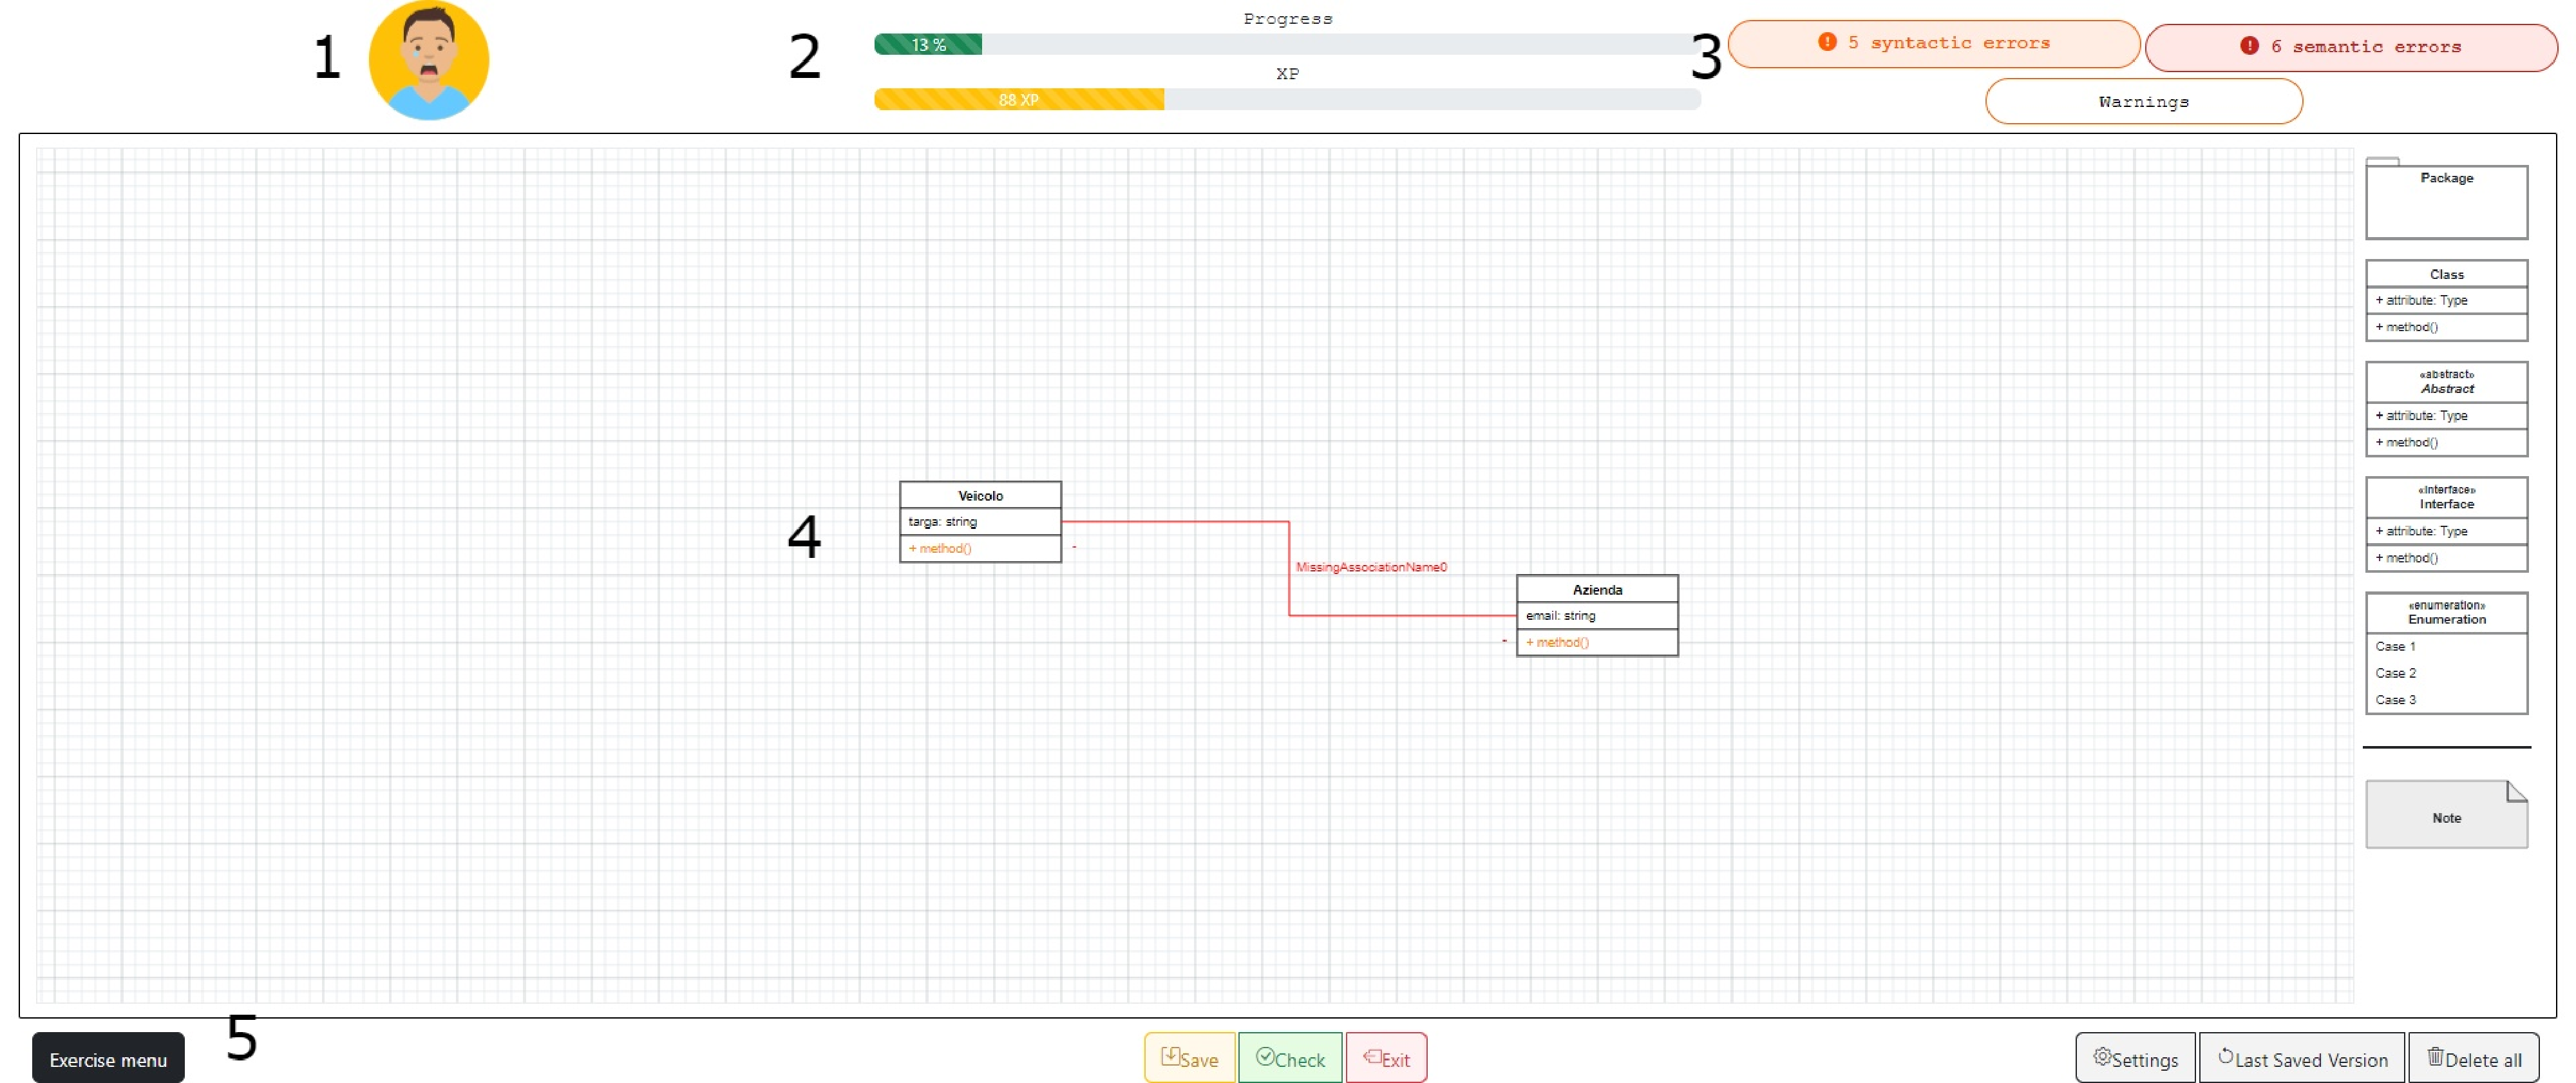
\includegraphics[width=1\linewidth]{Template_Latex_ScuDo_Tesi/Chapter4/exPage.pdf}
    \caption{Exercise page of the tool showing: 1) Student Avatar, 2) Indicators, 3) Error Lists, 4) Diagram Feedback, 5) Exercise Menu}
    \label{fig_tool}
\end{figure*}

\subsection{Evaluation Engine}

A second consequence of the empirical experiment, following the revision of all game mechanics, was the decision to reassess the implementation of the evaluation engine, with the end goal of identifying a set of rules, criteria, and practices independent from a specific modeling language, resulting in an evaluation approach that could be replicated in multiple software engineering disciplines. 

The development of the new evaluator had to address three main concerns that had emerged from the experiment:
\begin{enumerate}
    \item The original evaluator was excessively strict in multiple ways: the presence of a single solution, for example, would risk students having to \textit{guess} the correct elements to include in their diagrams, Additionally, correctness conditions kept into account neighboring elements, essentially forcing students to identify the correct names and types for all intended elements in order to succeed. The first necessary change for the new evaluator was to allow multiple solutions and multiple synonyms, increasing flexibility, and, most importantly, the removal of dependencies between elements as a condition for matching elements, making it a separate type of error.
    \item The feedback mechanism was among the most appreciated, but its implementation could still be improved: the original version would only show the correct elements, resulting in many scenarios where students saw no change in their diagram but still got penalized, and could not understand what their mistakes were. As a consequence, the new evaluator would need to identify errors beyond the absence of necessary elements, with a way to communicate them tied to the gamified feedback mechanism.
    \item Lastly, while the BIPMIN tool employed a distinction between syntactic and semantic errors, the corresponding feedback was kept separate, forcing students to address their syntax errors before the actual assessment, and with little explanations for why certain modeling choices were considered mistakes, resulting in a limiting and unexplained experience. It was decided to keep syntax and semantic errors separate and, at the same time, to expand the range of errors and feedback to ensure students could understand not only which elements had errors but the specific type and the actions needed to fix them as well; furthermore, the syntactic and semantic evaluation processes became sequential, with no reliance on passing the syntax check before element matching could be performed, to ensure complete feedback in a single evaluation step.  
\end{enumerate}

After identifying the necessary changes needed to implement the new evaluation engine, the subsequent step was to define a way to express the necessary requirements in an adequate data structure, as well as implementing a dedicated teacher interface for the creation of a reference structure compatible with said structure.

%The engine is deliberately exposed as a student-facing tool rather than a summative grading instrument: the rationale is that frequent, low-stakes feedback loops are more effective for learning than deferred, high-stakes assessment~\cite{marin2022}.

The data structure needed to implement the reference solution was defined by following an approach similar to how a human evaluator would assess a diagram: a human knows which are the necessary concepts that have to be represented in the diagram as classes (and their importance), knows the attributes each class can have with the allowed types and whether these attributes can also be a separate class, knows the associations between classes and the allowed multiplicity values in the pair, knows which relationships have more details such as inheritance between classes or association classes, and knows which classes, attributes, and associations between existing classes cannot be included. All this information was then converted into a data structure that can be easily expressed as a JSON file, allowing for easy importing, exporting, and editing, as well as creation and management through a web application; Table \ref{tab:solution_schema} summarizes the attributes of said data structure.

\begin{table}[ht]
  \centering
  \caption{Properties of the reference solution schema.}
  \label{tab:solution_schema}
  \small
  \begin{tabular}{lp{8cm}}
    \toprule
    \textbf{Element type} & \textbf{Required properties} \\
    \midrule
    Class & Canonical name; list of synonyms; weight (\textsc{strong} = mandatory, \textsc{weak} = optional); list of disallowed attribute names. \\
    Attribute & Canonical name; list of synonyms; list of allowed types; flag indicating whether the concept may alternatively be modeled as a separate class. \\
    Association & Canonical name; list of synonyms; source and destination class names; list of admissible multiplicity pairs. \\
    Intermediate class & Name of the bridging class; names of the two classes it connects. \\
    Generalisation & Parent class name; list of child class names. \\
    Forbidden class name & Names that should not appear as class labels (e.g., application-level concepts extraneous to the domain). \\
    Forbidden association name & Association labels that are disallowed (e.g., bare infinitive verbs). \\
    Forbidden pair & Pairs of class names that must not be directly connected. \\
    \bottomrule
  \end{tabular}
\end{table}

A reference solution can be created by a teacher using the dedicated section in the UMLegend tool, where it is possible to either draw a class diagram on the modeling canvas and create the corresponding data structure or to use a form where each element can be specified with all parameters. The process for creating a reference solution requires analytical skills and is composed of multiple steps: first of all, a textual description of a real-world application domain needs to be written, to identify the relevant concepts, with their attributes and relationships; then, the teacher should draw a tentative reference solution starting from the description, and in case multiple teachers are involved they should prepare a similar draft. All teachers involved can then compare all drafts and converge into at least one canonical solution, considering also synonyms for named elements, and one of them enters it in the tool using either the canvas or the form; if teachers agree that multiple reference solutions are valid then those are included as well.

This procedure is an activity that, depending on a given exercise's complexity, can grow to become time-consuming: a reasonable estimation is that, given a medium level exercise with around 30 to 45 total necessary elements, approximately one hour of work is needed per teacher, and in case multiple points of view are involved, at least one hour and a half of synchronization are needed, while entering the final solution is a relatively fast activity that takes less than 30 minutes, resulting in an average time of 3 hours needed to create complex exercises. While the time needed may make exercise creation seem like a tedious activity, it is a necessary investment, since the quality of the reference solution directly impacts the evaluation engine's ability to support automated feedback and, consequently, gamified learning.

Following the definition of the necessary data structure to implement reference solutions, the subsequent step was the definition of a new evaluation algorithm, keeping in mind the lessons learned from the empirical study. It was decided to divide the evaluation procedure in three steps: a first pass to evaluate the syntactic correctness of a diagram, to ensure that basic structural rules were followed; then, a semantic analysis focused on locating elements that match those described in the reference solution, to measure how well a student has represented the intended domain; lastly, a third assessment is performed, looking for elements and modeling choices that are not grave enough to be considered errors but still warrant a warning. 

The syntax evaluation analyzes all elements (classes, attributes, associations, intermediate classes) independently from the reference solution and assigns an error for each constraint that is violated (e.g., having no name or a duplicate name, using the wrong type for an attribute, not having multiplicity values or using an incorrect syntax for writing multiplicity values), making it possible for an element to have multiple errors and associated error messages in the feedback list; the sequence of steps, with the criteria evaluated for each type of element, are presented in Figure \ref{fig:syn_alg}. In case elements are found to have no name, the procedure assigns them a placeholder name to ensure subsequent steps that rely on naming can be performed. 


\begin{figure}[ht]
    \centering
    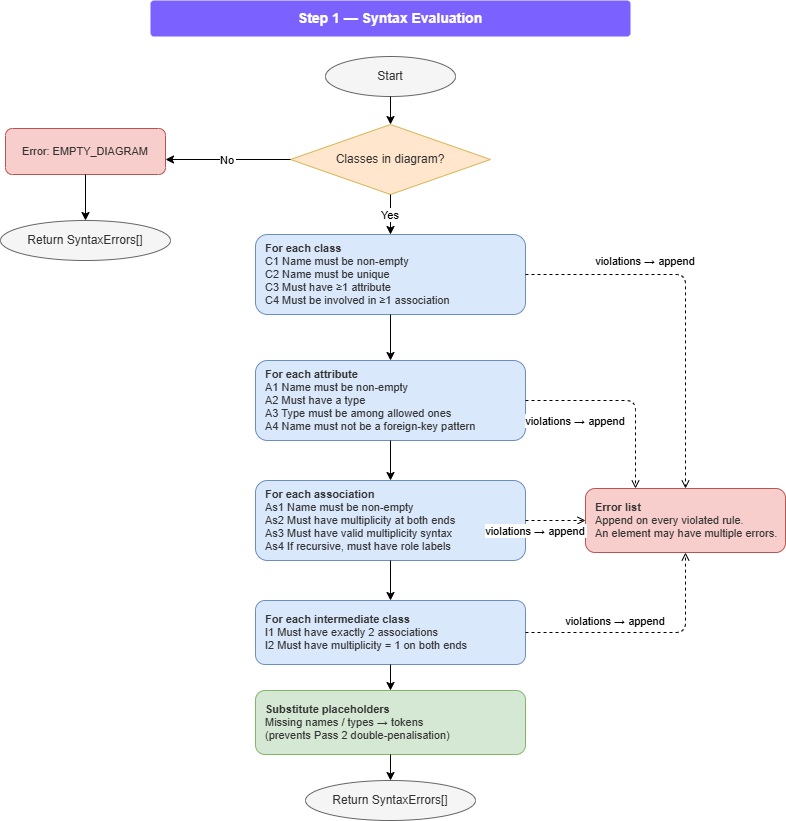
\includegraphics[width=0.75\linewidth]{syn_alg.png}
    \caption{Syntax evaluation algorithm}
    \label{fig:syn_alg}
\end{figure}

The semantic evaluation compares the student diagram against the reference solution, first looking for matches between reference elements and diagram elements according to their names: this is done by computing the \textit{normalized Levenshtein distance} between the diagram element's name and each reference element of the same type and its synonyms. A match is found if the distance between a diagram element's name and a reference name (or one synonym) is at most $0.25$, with the threshold being defined as such to tolerate writing errors and grammar mistakes. Elements that were found to have no name in the first step and thus received a placeholder name are not considered for evaluation in this step, to avoid assigning multiple errors to the same element.
After matches are found, subsequent assessments are performed on the matched elements to ensure domain details are also covered (e.g., attribute types, multiplicity values, association names), ensuring complete guidance for students; Figure \ref{fig:sem_alg} shows the steps that compose the algorithm for semantic evaluation.

\begin{figure}[ht]
    \centering
    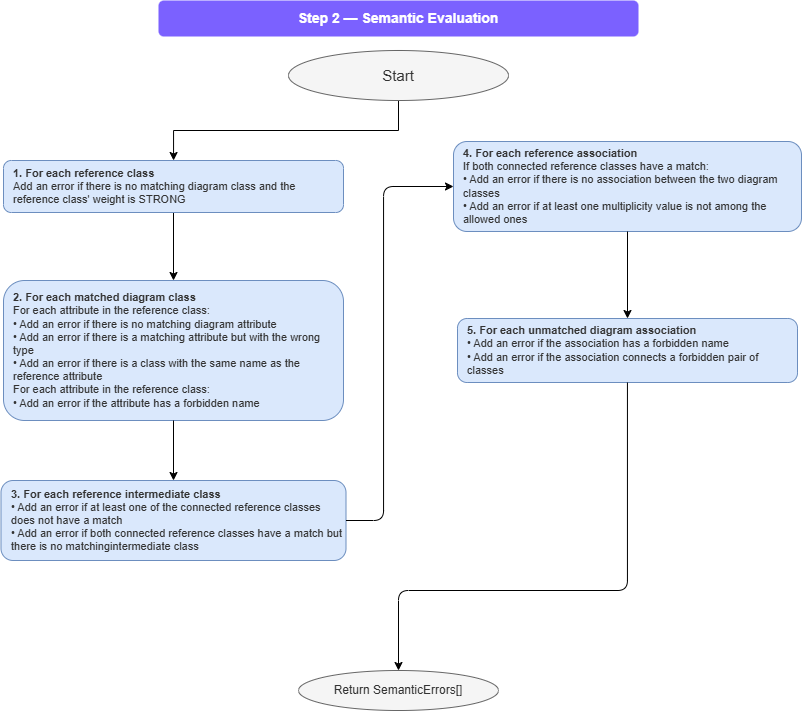
\includegraphics[width=0.75\linewidth]{sem_alg.png}
    \caption{Semantic evaluation algorithm}
    \label{fig:sem_alg}
\end{figure}

Lastly, the third step is used to identify minor modeling mistakes whose gravity is not high enough to consider them errors, but still count as design choices that can be improved; these mistakes are defined according to the pragmatic quality rules defined by Bolloju and Leung \cite{bolloju2006assisting}, and are reported to highlight issues that should be addressed but do not impact the completeness of the diagram. Figure \ref{fig:prag_alg} summarizes the pragmatic evaluation procedure applied at the end of each diagram check.

\begin{figure}[ht]
    \centering
    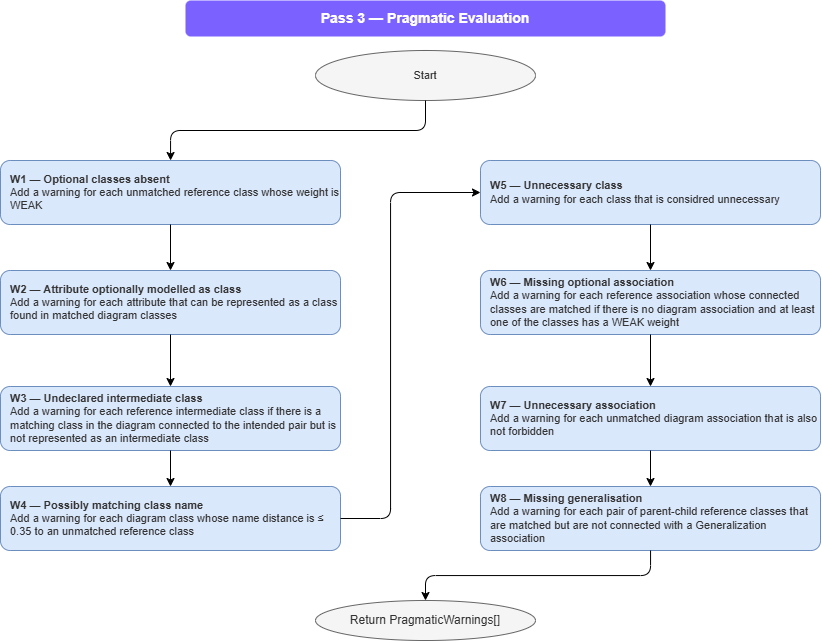
\includegraphics[width=0.75\linewidth]{prag_alg.png}
    \caption{Pragmatic evaluation algorithm}
    \label{fig:prag_alg}
\end{figure}


\section{Empirical Experiment with the Tool}

The development of UMLegend according to the new gamification framework was finalized in Autumn 2023, making it necessary to conduct a study to evaluate its effectiveness. Following the lessons learned from the BIPMIN experiment, it was decided to employ the tool in a single session first, to assess the effectiveness of the game mechanics on motivating the students and the tool's impact on learning performance, as well as to gather feedback before using the tool for the duration of a course. The experiment was conducted in January 2024 and followed a similar design to the one performed for evaluating BIPMIN: as such, the Goal-Question-Metric (GQM) template was adopted once again, expressing the purpose of the study as \textit{assess the impact of gamification on the production of UML class diagrams and their correctness from the point of view of Software Engineering teachers in the context of university courses}, with Table \ref{tab:gqm4} summarizing the experiment according to the template.


\begin{table}[ht]
  \rowcolors{2}{gray!25}{white}
\centering
\caption{GQM template for the experiment}
\label{tab:gqm4}
\small
\begin{tabular}{@{}p{0.3\columnwidth} p{0.55\columnwidth}@{}}
\toprule
Object of Study & Learning of UML Modeling \\
Purpose & Compare the traditional and gamified approach \\
Focus & Productivity, Correctness, Student Reception  \\
Context & Modeling tools \\
Perspective & Software engineering teachers \\
\bottomrule
\end{tabular}
\end{table}

\subsection{Study Design and Participants}

In the same vein as the 2023 experiment, participants were selected through convenience sampling among the students enrolled in the course \textit{Sistemi Informativi Aziendali}, offered as part of the Masters' Degree in Management Engineering, during the 2023-2024 academic year; participation was rewarded with 2 additional points on the exam grade, with assurance that participation was optional and that there would have been no consequences for not participating, or for participating in a suboptimal way. A total of 280 students took part in the study, split into 117 female students and 163 male students.

Contrary to the study performed in 2023, the experiment was conducted completely in presence at the end of the course, ensuring students had a sufficient level of modeling skill to perform adequately in the tasks; the UMLegend tool was served as a web application that students could access with their personal devices for the duration of the study.

Another similarity with the 2023 study was in the design of the experiment itself: the goal was to evaluate the differences between gamified and non-gamified UML class diagram modeling, and thus the within-subjects design was selected again. To allow for this comparison, a modified version of UMLegend was used for the study: while the long-term mechanics were kept in place for the entire study, the ability to mark exercises as non-gamified was added to the tool, and exercises marked as such offered no in-exercise mechanics and a less detailed feedback (e.g., a generic message stating that some classes were missing would be used rather than a separate message for each missing class).

The design was then set up to have students perform two exercises as tasks, solving one with the regular version and one with the non-gamified environment: the same 2x2 full factorial crossover design adopted for the original experiment was used in this scenario as well, keeping in mind the order of exercise and treatment as another variable and resulting in four possible combinations, which are presented in Table \ref{tab:exp_design}. Group assignment was random, resulting in four groups of 70 students.

\begin{table}[t]
  \rowcolors{2}{gray!25}{white}
\centering
\caption{Experiment Design for the 2024 UMLegend study}
\label{tab:exp_design}
\footnotesize
\begin{tabular}{@{}p{0.13\columnwidth} p{0.2\columnwidth} p{0.12\columnwidth} p{0.2\columnwidth} p{0.12\columnwidth}@{}}
\toprule
& \multicolumn{2}{c}{Task 1} & \multicolumn{2}{c}{Task 2} \\
& Exercise & Tool & Exercise & Tool \\
\midrule
Group 1 & Exercise 1 & Vanilla & Exercise 2 & Gamified \\
Group 2 & Exercise 1 & Gamified & Exercise 2 & Vanilla \\
Group 3 & Exercise 2 & Vanilla & Exercise 1 & Gamified \\
Group 4 & Exercise 2 & Gamified & Exercise 1 & Vanilla \\
\bottomrule
\end{tabular}%
\end{table}

The two exercises were selected among the ones offered as part of course exams held in past years and consisted of textual descriptions of real-life scenarios where a software application was to be implemented, requiring the design of a class diagram to support development. The exercises were estimated to have an average level of difficulty, ensuring that students close to the end of the course had a sufficient level of preparation to solve each of them in the allocated time window of 45 minutes.

After completing the two tasks, participants were asked to answer a questionnaire to measure their perception of the experience and of the game mechanics, as well as to gather opinions and feedback for improving the application.


\subsection{Research Questions and Metrics}

The following research questions were formulated to guide the experiment design:
\begin{itemize}
    \item \textbf{RQ1:} Does gamification improve the students' \textit{Productivity} in modeling UML class diagrams compared to non-gamified UML modeling?\\
    \emph{The reasoning behind this question is that gamification could provide a more engaging environment, leading students to make more changes in their diagrams and have them evaluated more frequently.}\\
    This question is further refined into:
    \begin{itemize}
        \item \textbf{RQ1.1:} Does the application of gamification impact the \textit{Size} of the diagrams made by the students?
        \item \textbf{RQ1.2:} Does the application of gamification impact the \textit{Attempts} made by students?
    \end{itemize}
    \item \textbf{RQ2:} Does gamification improve the \textit{Correctness} of the diagrams modeled by the students compared to non-gamified UML modeling?\\
    \emph{It is assumed that gamification could improve student performance by increasing diagram completeness and reducing the errors made by the students.}\\
    This question is further refined into:
    \begin{itemize}
        \item \textbf{RQ2.1:} Does the application of gamification impact the \textit{Completeness} of the diagrams produced by the students?
        \item \textbf{RQ2.2:} Does the application of gamification impact the \textit{Errors} found in the diagrams produced by the students?
    \end{itemize}
    \item \textbf{RQ3:} What is the students' \textit{Perception} of gamified UML modeling?\\
    \emph{The rationale behind this question is that gamification is positively perceived by the students with more involvement and willingness to adopt it.}\\
    This question is further refined into:
    \begin{itemize}
        \item \textbf{RQ3.1:} What is the perceived usability of the gamified UML modeling tool?
        \item \textbf{RQ3.2:} What is the appreciation of the gamified characteristics and mechanics in the gamified UML modeling tool?
        \item \textbf{RQ3.3:} What are the issues and improvement areas for the gamified UML modeling tool?
    \end{itemize}
\end{itemize}

Due to the experiment design remaining unchanged from the 2023 experiment, independent variables observed for analysis in the new study remained the same: the \textit{Treatment}, that is, the use of the gamified or non-gamified modeler, remained the main independent variable under scrutiny, while other independent variables considered as possible confounding factors were the \textit{Exercise} used as task and the \textit{Group} to which participants were assigned.

Independent variables were considered for research questions RQ1 and RQ2, since they dealt with data that could be analyzed with statistical methods, while metrics related to RQ3 were connected with the final questionnaire, and were analyzed with a qualitative approach. The collection of dependent variables was performed automatically with the tool: each evaluation launched by a students would record the current diagram and the state of game mechanics, with both the regular version and the non-gamified one. 

To answer RQ1, two dependent variables were considered: first, the \textit{Size} of submitted diagrams, computed as the count of classes, attributes, and associations, was recorded, with the assumption that adopting gamification would lead to significant changes in the number of elements present in a student's diagram, with the size of the reference solution adopted for the study as the target value. The second variable considered was the number of \textit{Attempts}, that is, the number of evaluations launched by a student during each task; this metric was collected for both the Vanilla and Gamified version, and was measured with the assumption that using gamification would lead students to perform more evaluations for their exercises. In the Vanilla version, changes in the obtainable experience points and in the diagram completeness score, as well as the count of errors, are still computed internally and stored despite not being shown to students.


The dependent variables selected to answer RQ2 were split according to the refined sub-questions: for RQ2.1, the \textit{Completeness} of diagrams was considered, with the reason being that adopting gamification would guide students to make significant improvement, and thus increase this metric; for RQ2.2, instead, three metrics were computed as the count of syntactic and semantic errors, as well as pragmatic warnings obtained with the final submitted diagram, with the assumption that gamification would have a positive effect and lead to a decrease in such counts.

The final questionnaire consisted of multiple sets of questions, with each set being focused around a specific sub-question. To answer RQ3.1, which aimed at assessing the overall student perception of the gamified experience, questions taken from the Technology Acceptance Model (TAM) \cite{lee2003technology} and GAMEX \cite{eppmann2018gameful} questionnaires were used. The GAMEX questionnaire was used in the same fashion as in the first BIPMIN study, to measure the six different aspects that characterize a gamified experience, while the TAM questionnaire was adopted to assess the overall student perception of the tool, measuring four high-level constructs such as Perceived Usefulness (PU, the belief that using an application would improve performance), Perceived Ease of Use (PE, the belief that using an application requires little physical and mental effort), Behavioral Intention to Use (BI, the measure of how much one would be inclined to use an application in a specific way), and Attitude Towards Usage (ATU, the measure of how much one would want to use an application). Answers to both questionnaires were expressed through a Likert scale going from a score of 1 (Strongly Disagree) to 5 (Strongly Agree).

To answer RQ3.2, a specific set of questions was created, centered around each of the implemented game mechanics: the same five questions were repeated for each mechanic, assessing the students' opinions about its perceived usefulness, influence in using the application, satisfaction, motivating effect, and distracting effect. Answers to these questions were expressed with the same Likert scale format used for the TAM and GAMEX.

Lastly, two open questions were included to answer RQ3.3, which students could use to report issues encountered during the study and to leave suggestions for improving the tool. 

%The data is available as an online resource\footnote{\url{https://doi.org/10.6084/m9.figshare.25968082.v2}}. 

\subsection{Analysis Method}
To answer the sub-questions derived from RQ1 and RQ2, the following null hypotheses were formulated:
\begin{itemize}
    \item \emph{${H_{s_{0}}}$:} The application of gamification has no statistically significant impact on the size of the diagrams produced by the students
    \item \emph{${H_{as_{0}}}$:} The application of gamification has no statistically significant impact on the number of attempts (diagram evaluations) made by the students
    \item \emph{${H_{pr_{0}}}$:} The application of gamification has no statistically significant impact on the completeness of the diagrams produced by the students
    \item \emph{${H_{syn_{0}}}$:} The application of gamification has no statistically significant impact on the number of syntax errors made by students
    \item \emph{${H_{sem_{0}}}$:} The application of gamification has no statistically significant impact on the number of semantic errors made by students
    \item \emph{${H_{prag_{0}}}$:} The application of gamification has no statistically significant impact on the number of pragmatic warnings raised by students
\end{itemize}

Assuming that the variables would not follow a normal distribution, it was decided to test these hypotheses using a non-parametric approach; the statistical method adopted was, according to the standard practice for conducting full factorial crossover experiments \cite{vegas2016crossover}, a repeated measures linear mixed model (ANOVA), comparing each metric separately depending on the the treatment, with the exercise and the group assignment being considered confounding factors that could threaten the validity of the results.

Furthermore, the significance level was adjusted with the application of Bonferroni correction to account for multiple comparisons and to counteract the risk of multiple statistical tests increasing the change of false positives; given a total of six statistical tests being conducted in the analysis, the p-value threshold was adjusted, with $\alpha_C = \alpha / n =  0.0083$ being needed to imply statistical significance. 


Lastly, RQ3 was evaluated with a questionnaire whose answers could not be analyzed with statistical hypothesis testing; as a consequence, descriptive statistics were used to answer RQ3.1 and RQ3.2. The approach used was to compute, for each group of questions related to the same topic (e.g., Perceived Usefulness for the TAM, Enjoyment for the GAMEX, or a given game mechanic) the average score, rounded down, given by each student as the representation of said student's opinion. The distribution of opinions was then reported with stacked diverging bar charts, to rank each questionnaire's constructs and measure the overall perception.

RQ3.3, instead, was analyzed using open-ended questions and, as such, a similar procedure as the one used for the BIPMIN study was performed, adopting the \textit{open coding} approach defined by the Straussian Grounded Theory approach.

The goal of the analysis was to identify topics in the students' answers and then to group answers to identify common topics and opinions; the coding process involved the analysis of each answer one by one to identify the most compatible topic among the existing one, tagging the question with the topic if one was found, or creating a new, suitable one otherwise, resulting in the creation of the topic set. After all answers had been analyzed once, they were all reviewed a second time to ensure the original topic was still suitable or if there was another, more relevant one to tag the answer with; following that, a final review was performed to locate answers that fit more than one topic, resulting in certain answers having more than one relevant topic.

\subsection{Results}

The summary statistics for RQ1-related metrics, that is, the size of the final saved diagram and the number of checks performed for each exercise, are reported in in Table \ref{tab:rq1_4}. These statistics (minimum, maximum, mean, median, standard deviations) have been computed separately depending on the treatment, and Figure \ref{fig:rq1_4} shows a combined box and violin plot that represents their distribution.

\begin{table}[htbp]
  \rowcolors{2}{gray!25}{white}
    \small
    \centering
    \caption{Maximum, Minimum, Average, and Median scores for \textit{Productivity} metrics}
    \begin{tabular}{lrrrr}
    \toprule
    & Min & Max & Mean (SD) & Median \\
    \midrule
    Size (V)& 9 & 64 & 34.61 (9.09) & 33 \\
    Size (G) & 3 & 69 & 34.18 (9.40) & 32 \\
    Attempts (V) & 0 & 35 & 5.68 (5.00) & 3 \\
    Attempts (G) & 1 & 43 & 6.66 (7.16) & 4 \\
    \bottomrule
    \end{tabular}
    \label{tab:rq1_4}
\end{table}


\begin{figure}[H]
    \centering
    \begin{subfigure}{0.7\linewidth}
        \centering
        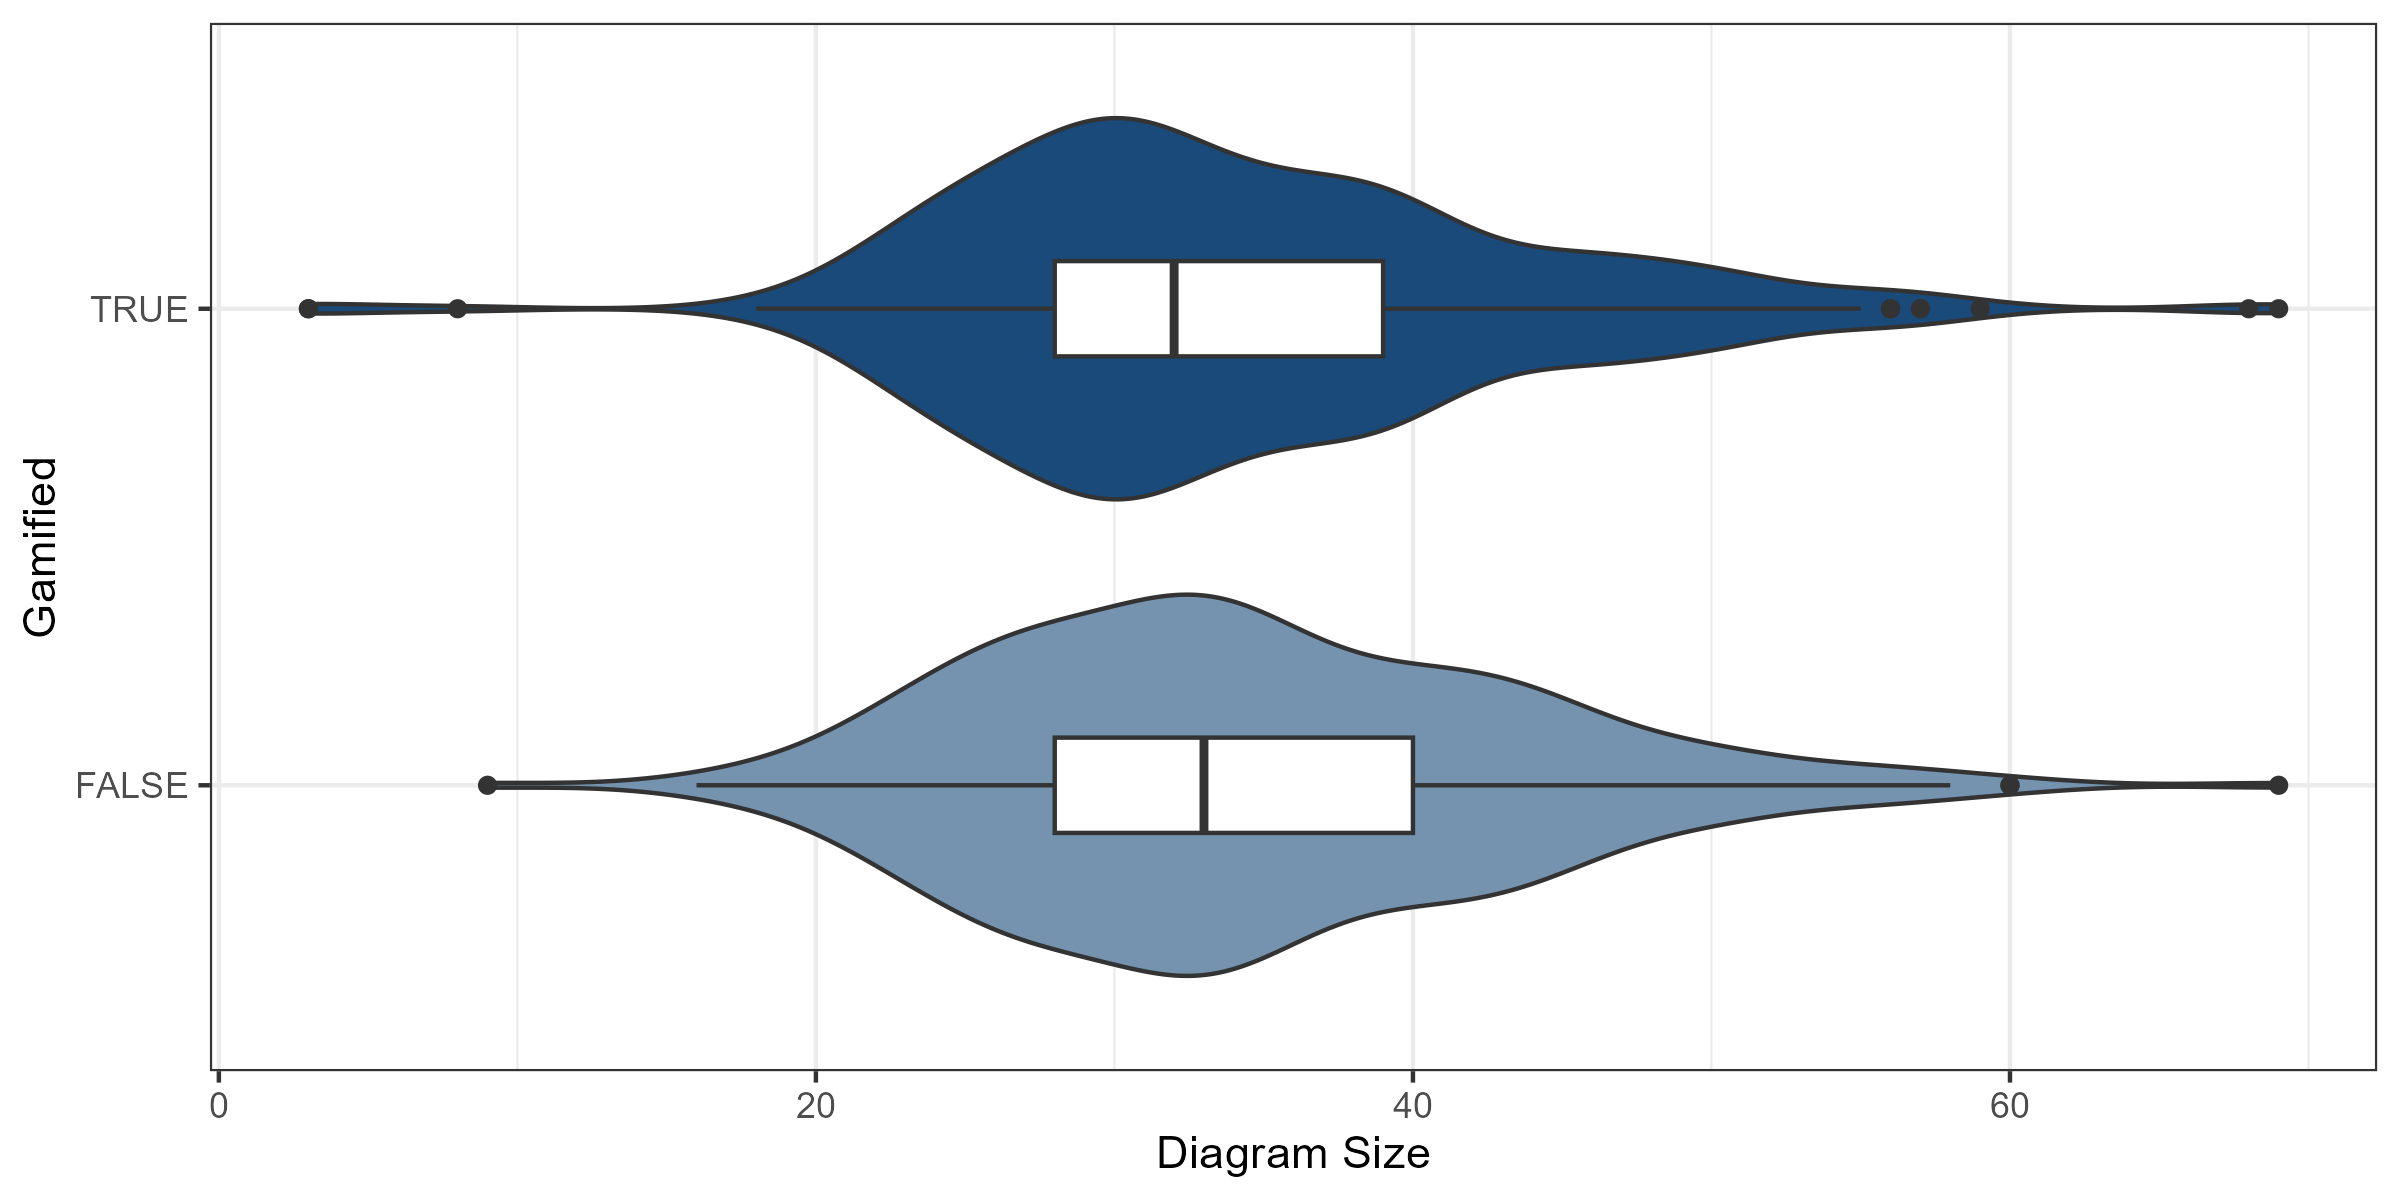
\includegraphics[width=\linewidth]{Template_Latex_ScuDo_Tesi/Chapter4/size_violin.png}
        \caption{Box and violin plot for the \textit{Size} metric}
        \label{fig:rq1_size}
    \end{subfigure}\hfill
    \begin{subfigure}{0.7\linewidth}
        \centering
        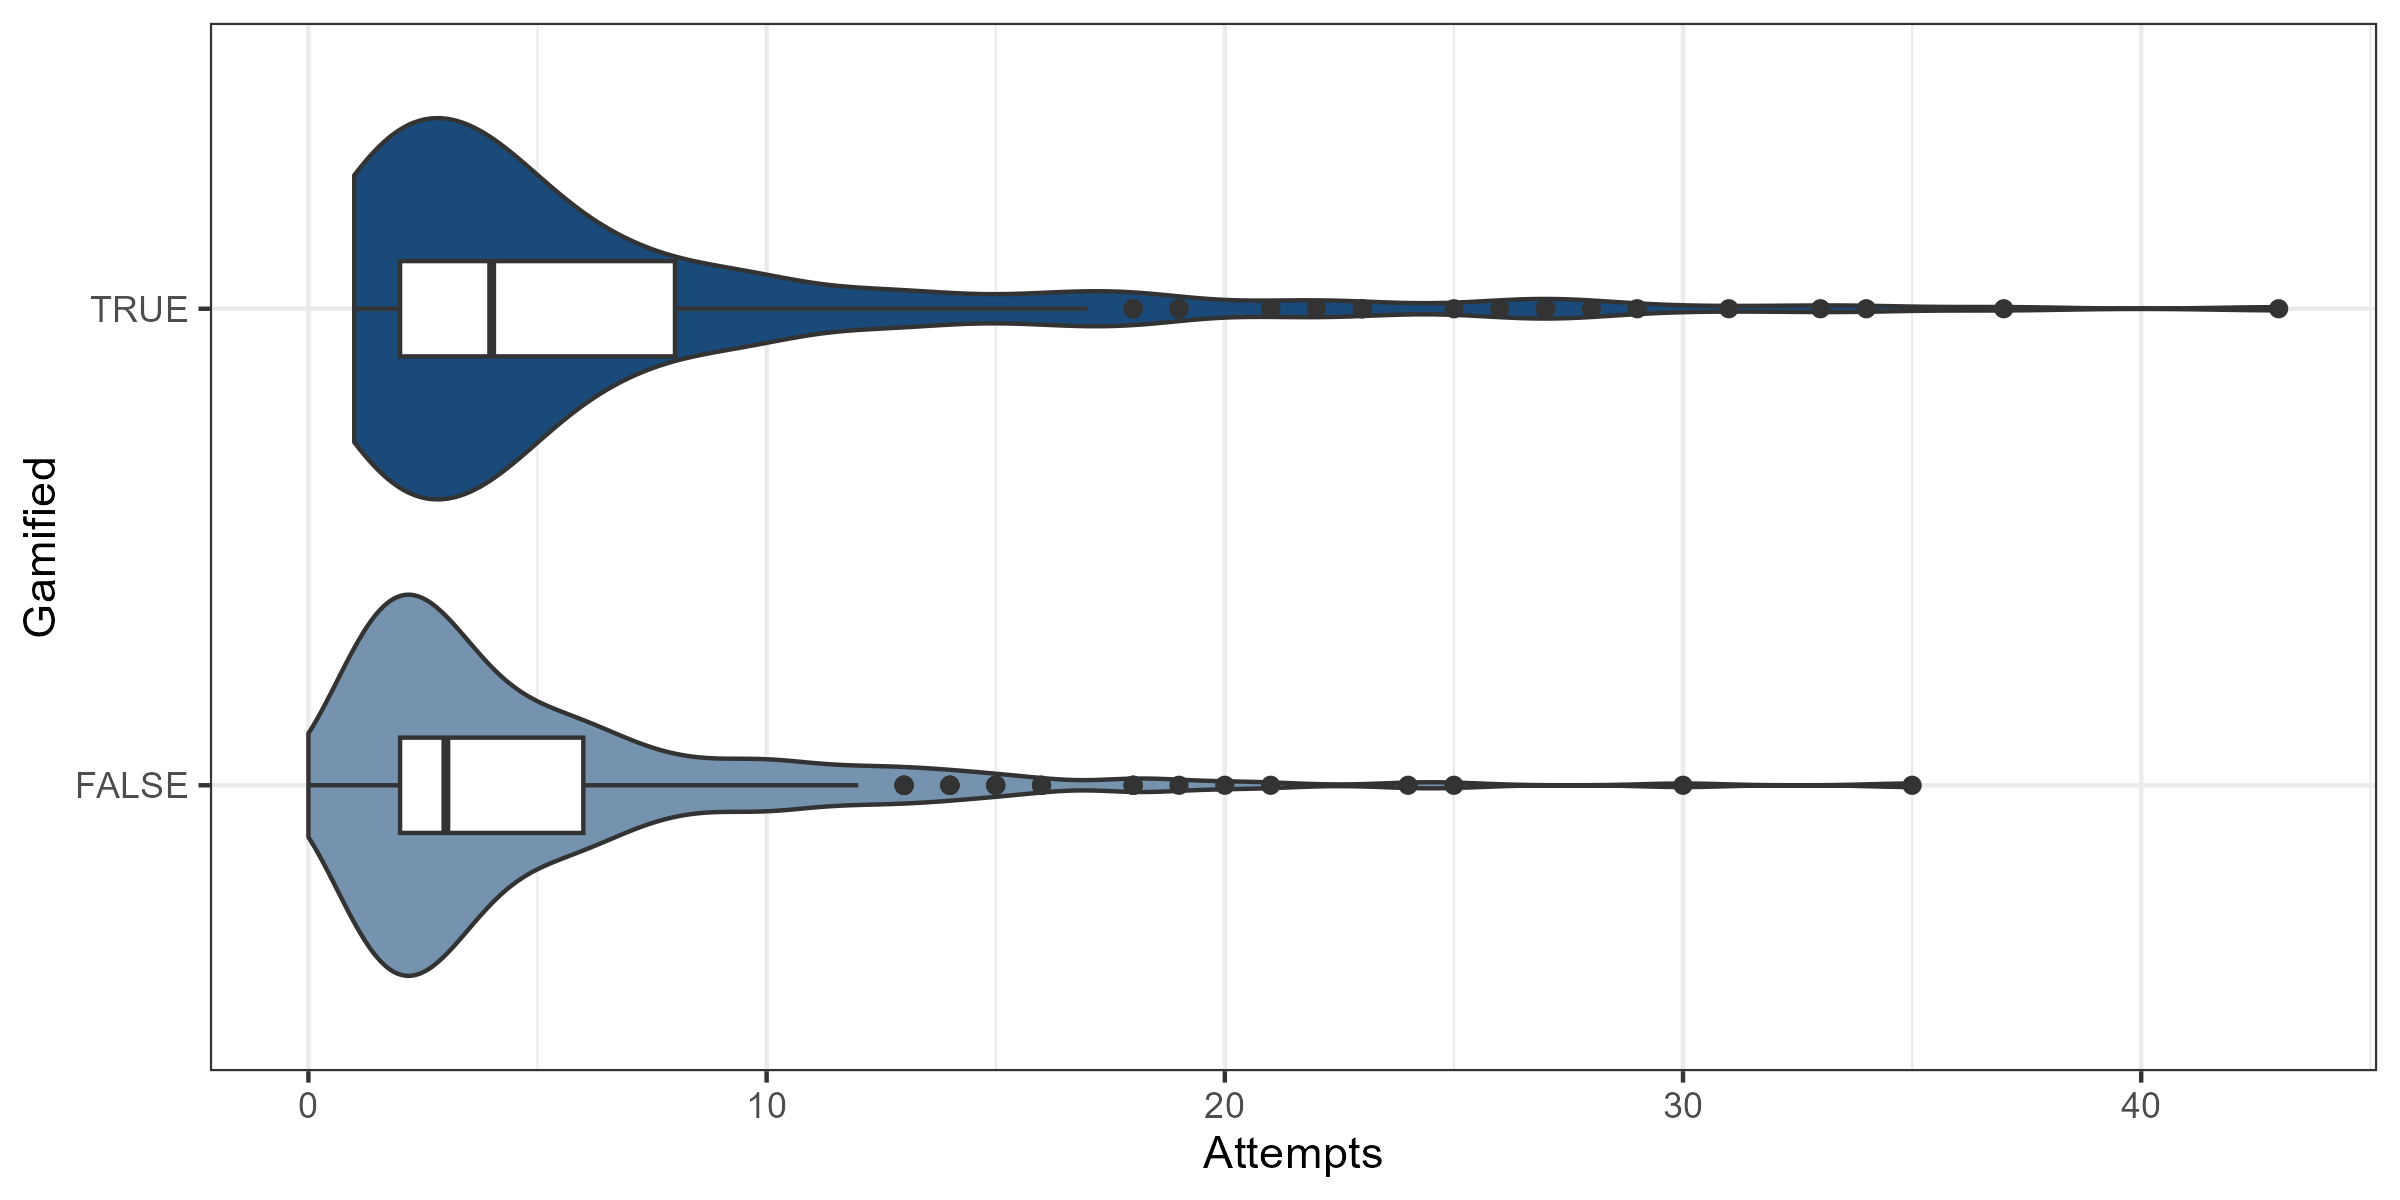
\includegraphics[width=\linewidth]{Template_Latex_ScuDo_Tesi/Chapter4/attempts_violin.png}
        \caption{Box and violin plot for the \textit{Attempts} metric}
        \label{fig:rq1_attempts}
    \end{subfigure}
    \caption{Box and violin plots for RQ1 metrics}
    \label{fig:rq1_4}
\end{figure}

For what concerns \textit{Size}, the plot shows that the distribution is more or less equal, with the mean value being slightly higher for the non-gamified version, implying that students produce less dense diagrams when using gamification. \textit{Attempts} achieved a different result, with a higher number of checks being performed on average with the gamified version, and overall higher numbers compared to the Vanilla version. A possible implication is that gamification does may not lead students to make significant changes, but it could be a guiding factor in performing more automated assessments.

An ANOVA test was performed on the two Productivity metrics and their distribution to answer RQ1 and possibly reject the two null hypotheses, with the goal of identifying a statistically significant impact of gamification on student productivity; Table \ref{tab:rq1_4_anova} presents, for each metric and the corresponding hypothesis, the results of the ANOVA test according to the main factor (gamification against no gamification) and the two confounding factors (exercise and the combination of treatment and exercise).


\begin{table}[ht]
  \rowcolors{2}{gray!25}{white}
\footnotesize
\centering
\begin{tabular}{lcccc}
    \toprule
         Factor / vars:& 
         \multicolumn{2}{c}{Size (${H_{s_{0}}}$)} & \multicolumn{2}{c}{Attempts (${H_{as_{0}}}$)} \\
         & coeff. & p-value & coeff. & p-value \\
    \midrule
    Treatment & -0.436 & 0.577 & 1.589 & \textbf{2.45e-03} \\
    Exercise & -8.3429 & \textbf{$\lt$ 2e-16} & 0.2964 & 0.574 \\
    Group & 0.1614 & 0.644 & -0.3107 & 0.187 \\
    \bottomrule
    \end{tabular}
\caption{Results of the statistical analysis for RQ1 metrics: Size and Attempts. Statistically significant p-values are in bold ($\alpha = 0.0083$)}
\label{tab:rq1_4_anova}
\end{table}


The analysis considers the non-gamified version as the reference one, confirming what was highlighted by Figure \ref{fig:rq1_4}: gamification leads to slightly smaller diagrams but a higher number of evaluations, encouraging students to interact more and more with the game mechanics.

The p-value associated with \textit{Size} is not statistically significant and, consequently, the null hypothesis ${H_{s_{0}}}$ cannot be rejected: gamification does not impact the size of student-made diagrams in any way, and as a consequence does not lead students to make significant changes.

Conversely, the p-value obtained by comparing the average number of \textit{Attempts} is statistically significant, implying that gamification does have an impact on the metric: with the average number of submissions being higher with the gamified version it is possible to reject hypothesis ${H_{as_{0}}}$ and affirm that gamification has a positive effect on the students' tendance to automatically evaluate diagram and, as a consequence, on their overall commitment.

For what concerns confounding factors, the only statistically significant result is that \textit{Size} depends on the exercise: the analysis took the first exercise as reference, and the negative value of the coefficient implies that the second exercise had a much lower size on average (30.23 against 38.57); as a point of comparison, the reference solution for the two exercises had a total size of 43 elements and 32 elements respectively. The difference in average sizes obtained by the students is in line with the fact that the two exercises also require different elements to be considered correct; however, this difference could also imply that one exercise required more effort to fully represent the intended domain and, consequently, be more complex than the other.


\answer{RQ1}{Applying gamification to class diagram exercises had no impact on the diagram size, implying that it does not encourage students to make significant changes to their diagrams but, possibly, to edit the existing elements to make them fit the context. The statistically significant increase on the number of attempts, instead, can be seen as a positive effect of gamification, since it means that tying the evaluation to the game mechanics makes students more inclined to evaluate their solution, making it reasonable to assume a positive effect on student commitment. Productivity metrics were relatively not impacted by other factors involved in the study design, with the only significant effect being on diagram size depending on the exercise: with one exercise having a lower element count, on average, it may be possible that one exercise was easier, impacting the validity of the study.}

To answer RQ2, diagram completeness and the count of errors (syntactic, semantic, and pragmatic warnings) were collected through the tool; Table \ref{tab:rq2_4} lists the minimum, maximum, mean, median, and standard deviation for these four metrics depending on the two treatment, while Figure  shows the combined box and violin plots for the distribution of the four metrics, also according on the use of gamification or not.

\begin{table}[htbp]
  \rowcolors{2}{gray!25}{white}
    \footnotesize
    \centering
    \caption{Maximum, Minimum, Average, and Median scores for correctness metrics}
    \begin{tabular}{lrrrr}
    \toprule
    & Min & Max & Mean (SD) & Median \\
    \midrule
    Completeness (V) & 0 & 98 & 42.54 (13.09) & 44  \\
    Completeness (G) & 9 & 95 & 47.21 (13.18) & 46 \\
    Syntax Errors (V) & 0 & 31 & 5.4 (6.48) & 3 \\
    Syntax Errors (G) & 0 & 32 & 3.79 (5.51) & 1 \\
    Semantic Errors (V) & 2 & 18 & 9.64 (2.91) & 9 \\
    Semantic Errors (G) & 2 & 18 & 8.71 (2.69) & 8 \\
    Pragmatic Warnings (V) & 0 & 8 & 2.05 (1.54) & 2 \\
    Pragmatic Warnings (G) & 0 & 10 & 2.20 (1.61) & 2 \\
    \bottomrule
    \end{tabular}
    \label{tab:rq2_4}
\end{table}

\begin{figure}[H]
    \centering
    \begin{subfigure}{0.5\linewidth}
        \centering
        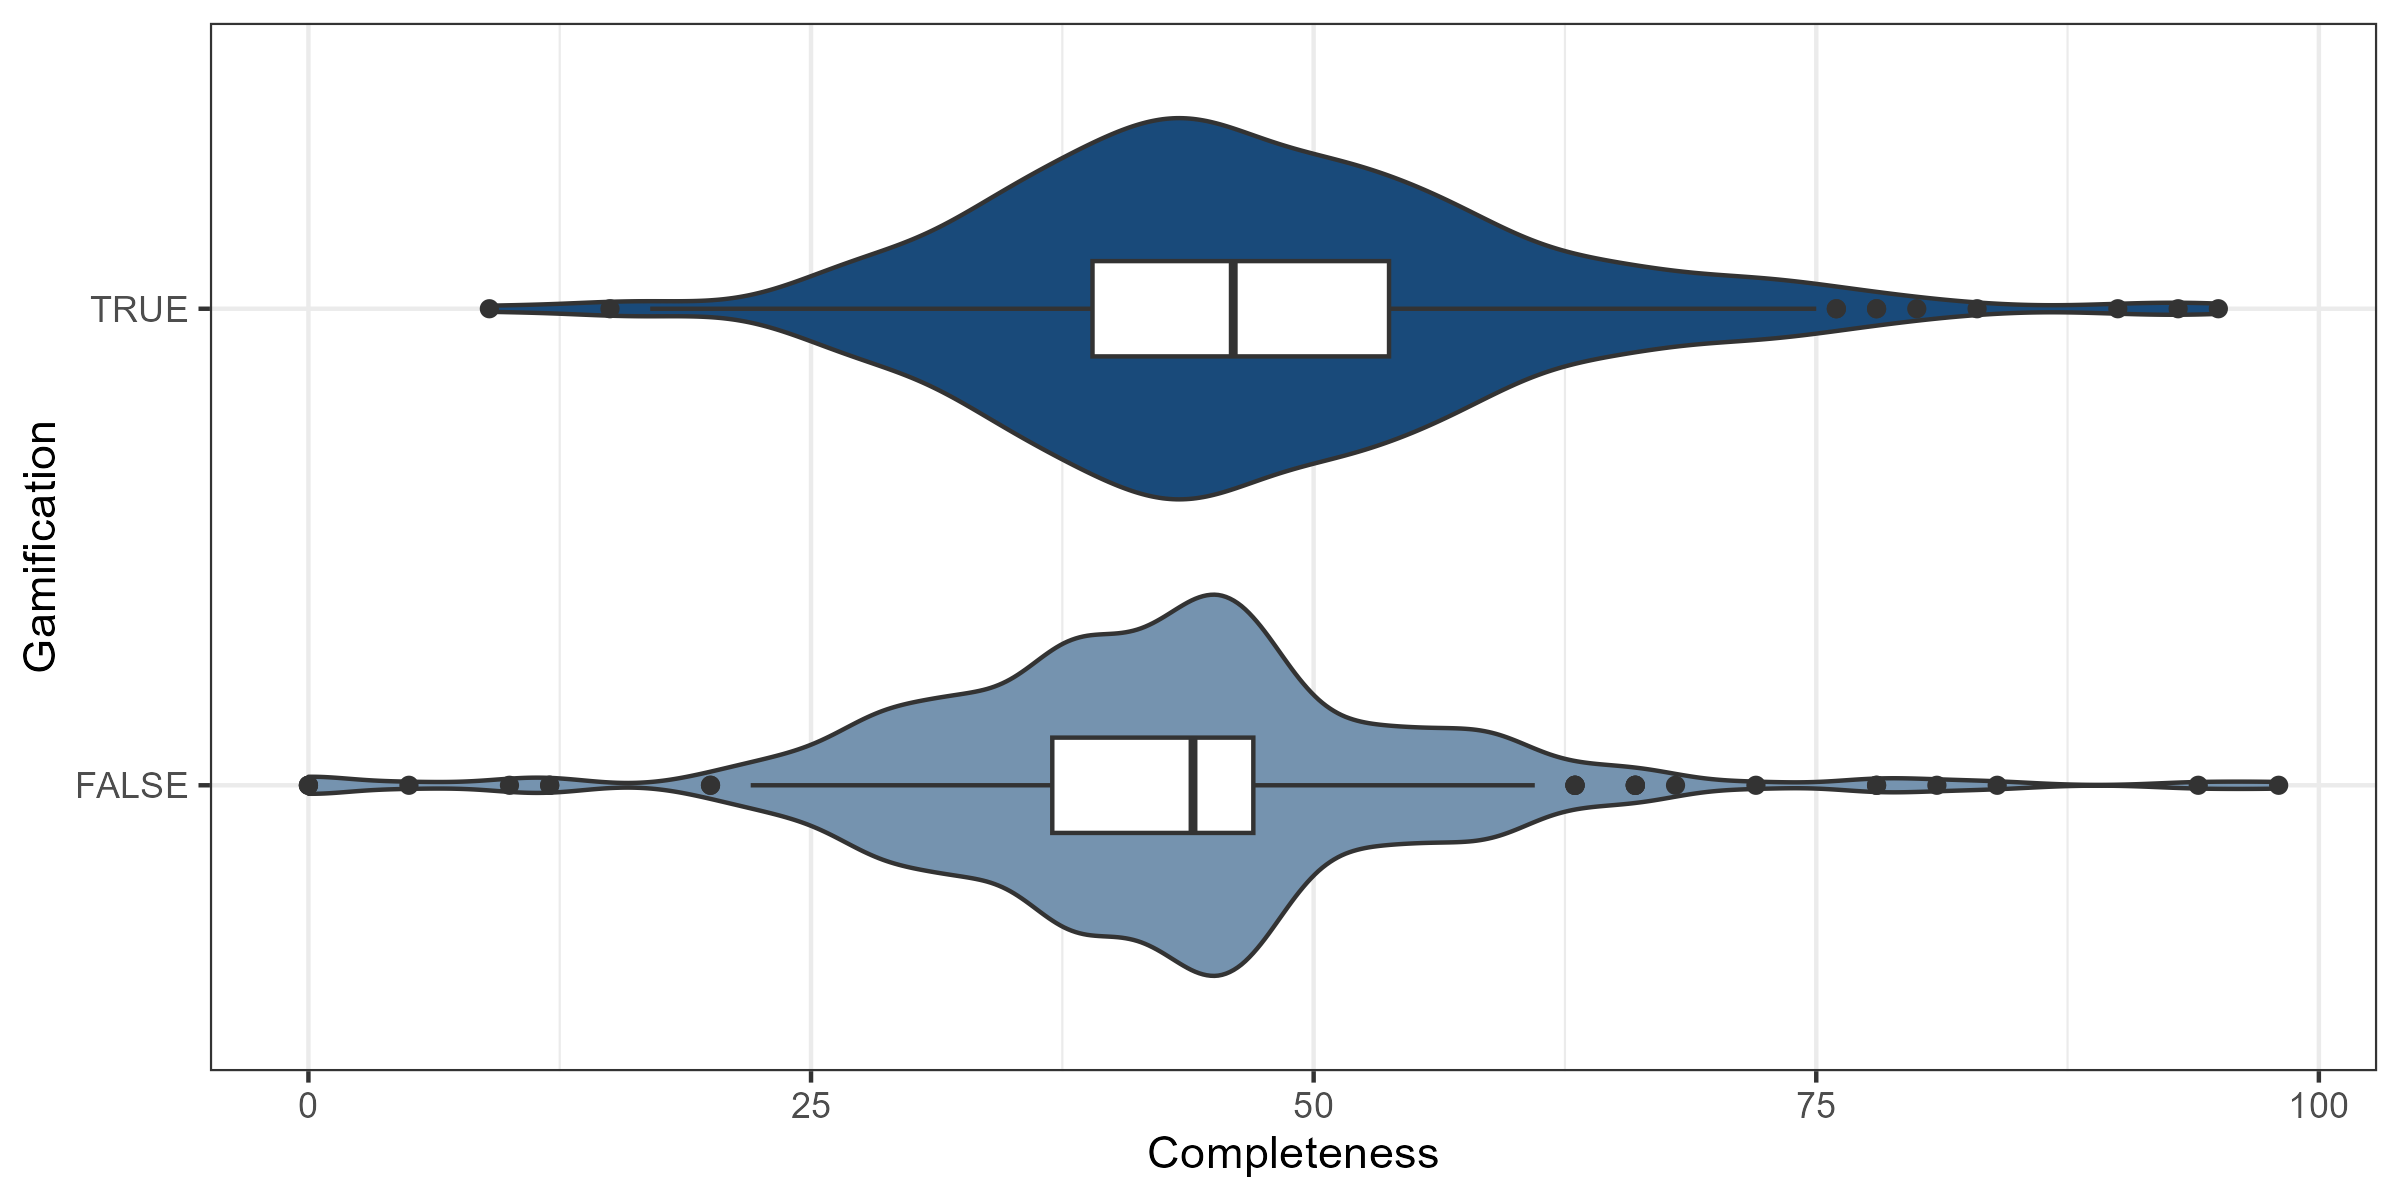
\includegraphics[width=\linewidth]{Template_Latex_ScuDo_Tesi/Chapter4/compl_violin.png}
        \caption{Box and violin plot for the \textit{Completeness} metric}
        \label{fig:rq2_compl}
    \end{subfigure}\hfill
    \begin{subfigure}{0.5\linewidth}
        \centering
        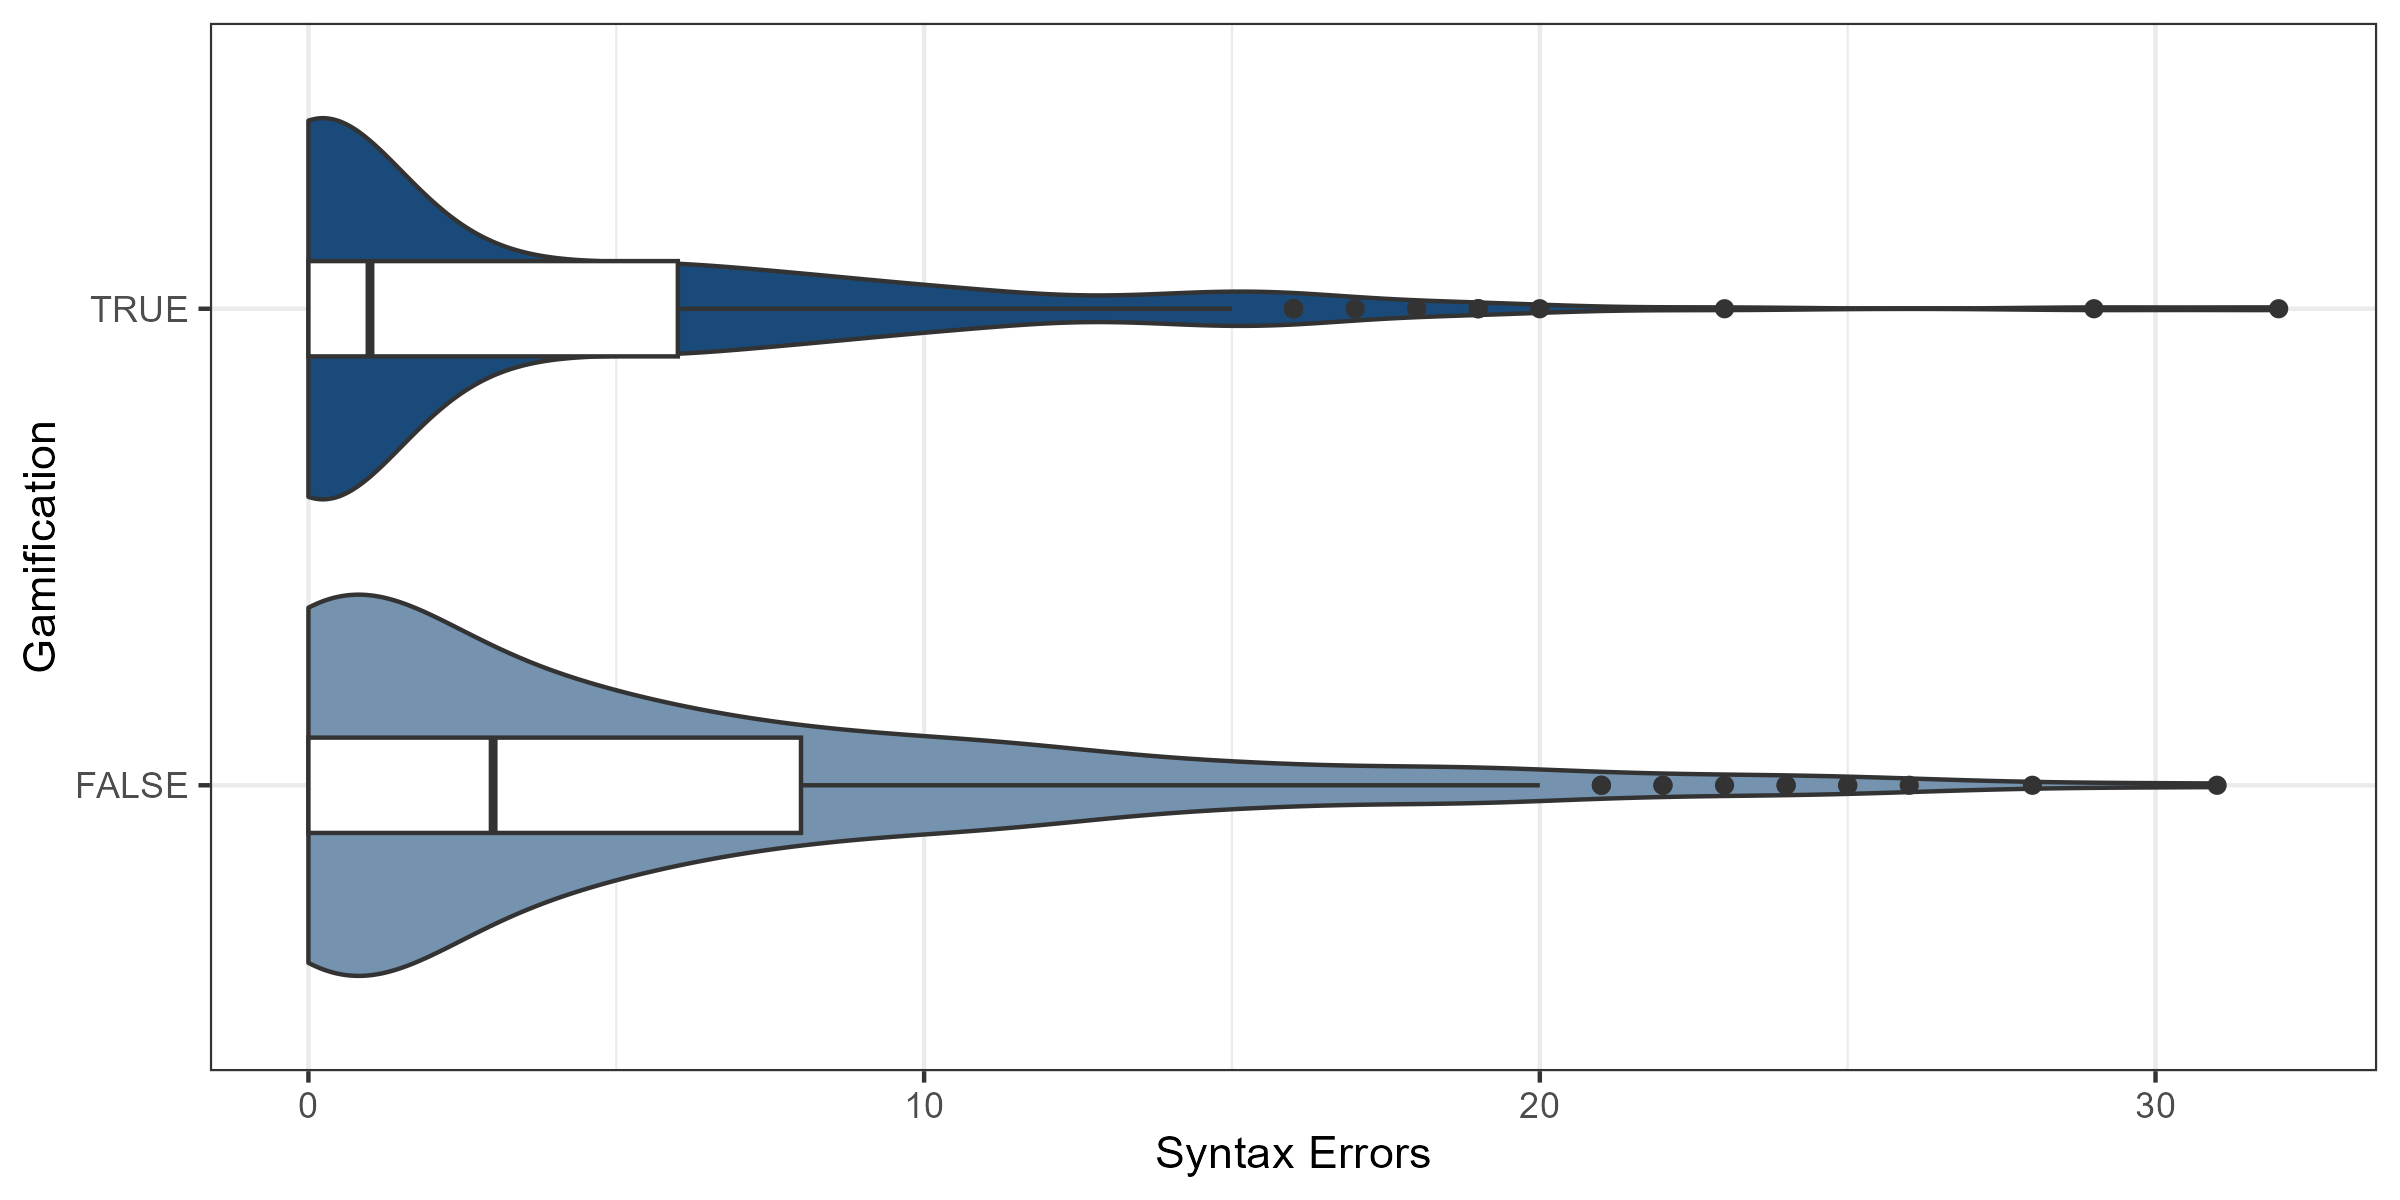
\includegraphics[width=\linewidth]{Template_Latex_ScuDo_Tesi/Chapter4/syn_violin.png}
        \caption{Box and violin plot for the \textit{Syntax Errors} metric}
        \label{fig:rq2_syn}
    \end{subfigure}\hfill
    \begin{subfigure}{0.5\linewidth}
        \centering
        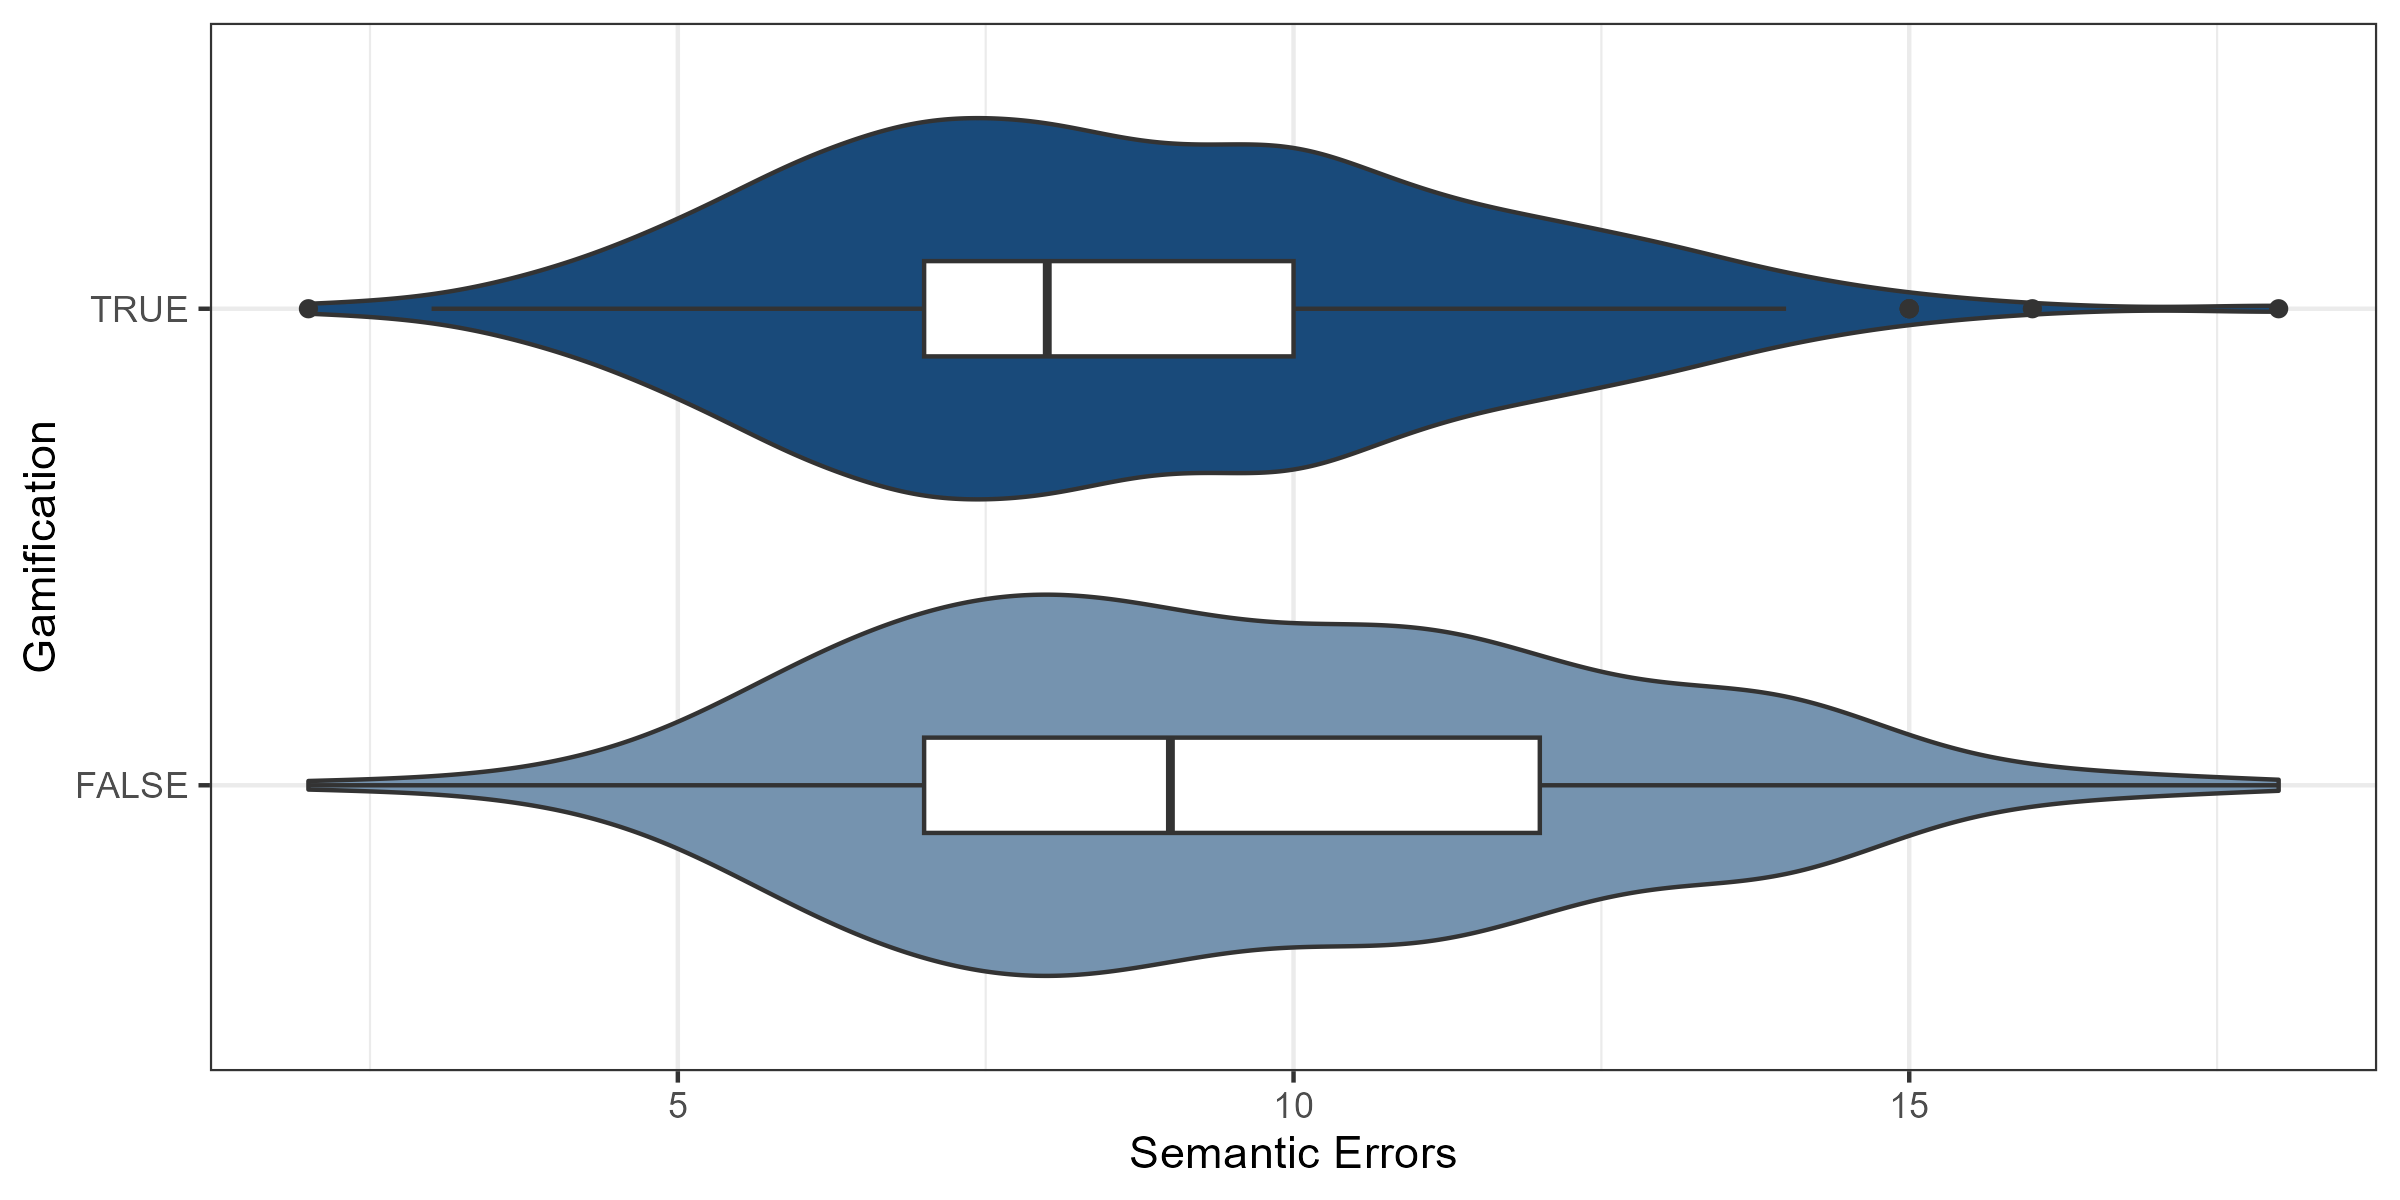
\includegraphics[width=\linewidth]{Template_Latex_ScuDo_Tesi/Chapter4/sem_violin.png}
        \caption{Box and violin plot for the \textit{Semantic Errors} metric}
        \label{fig:rq2_sem}
    \end{subfigure}\hfill
    \begin{subfigure}{0.5\linewidth}
        \centering
        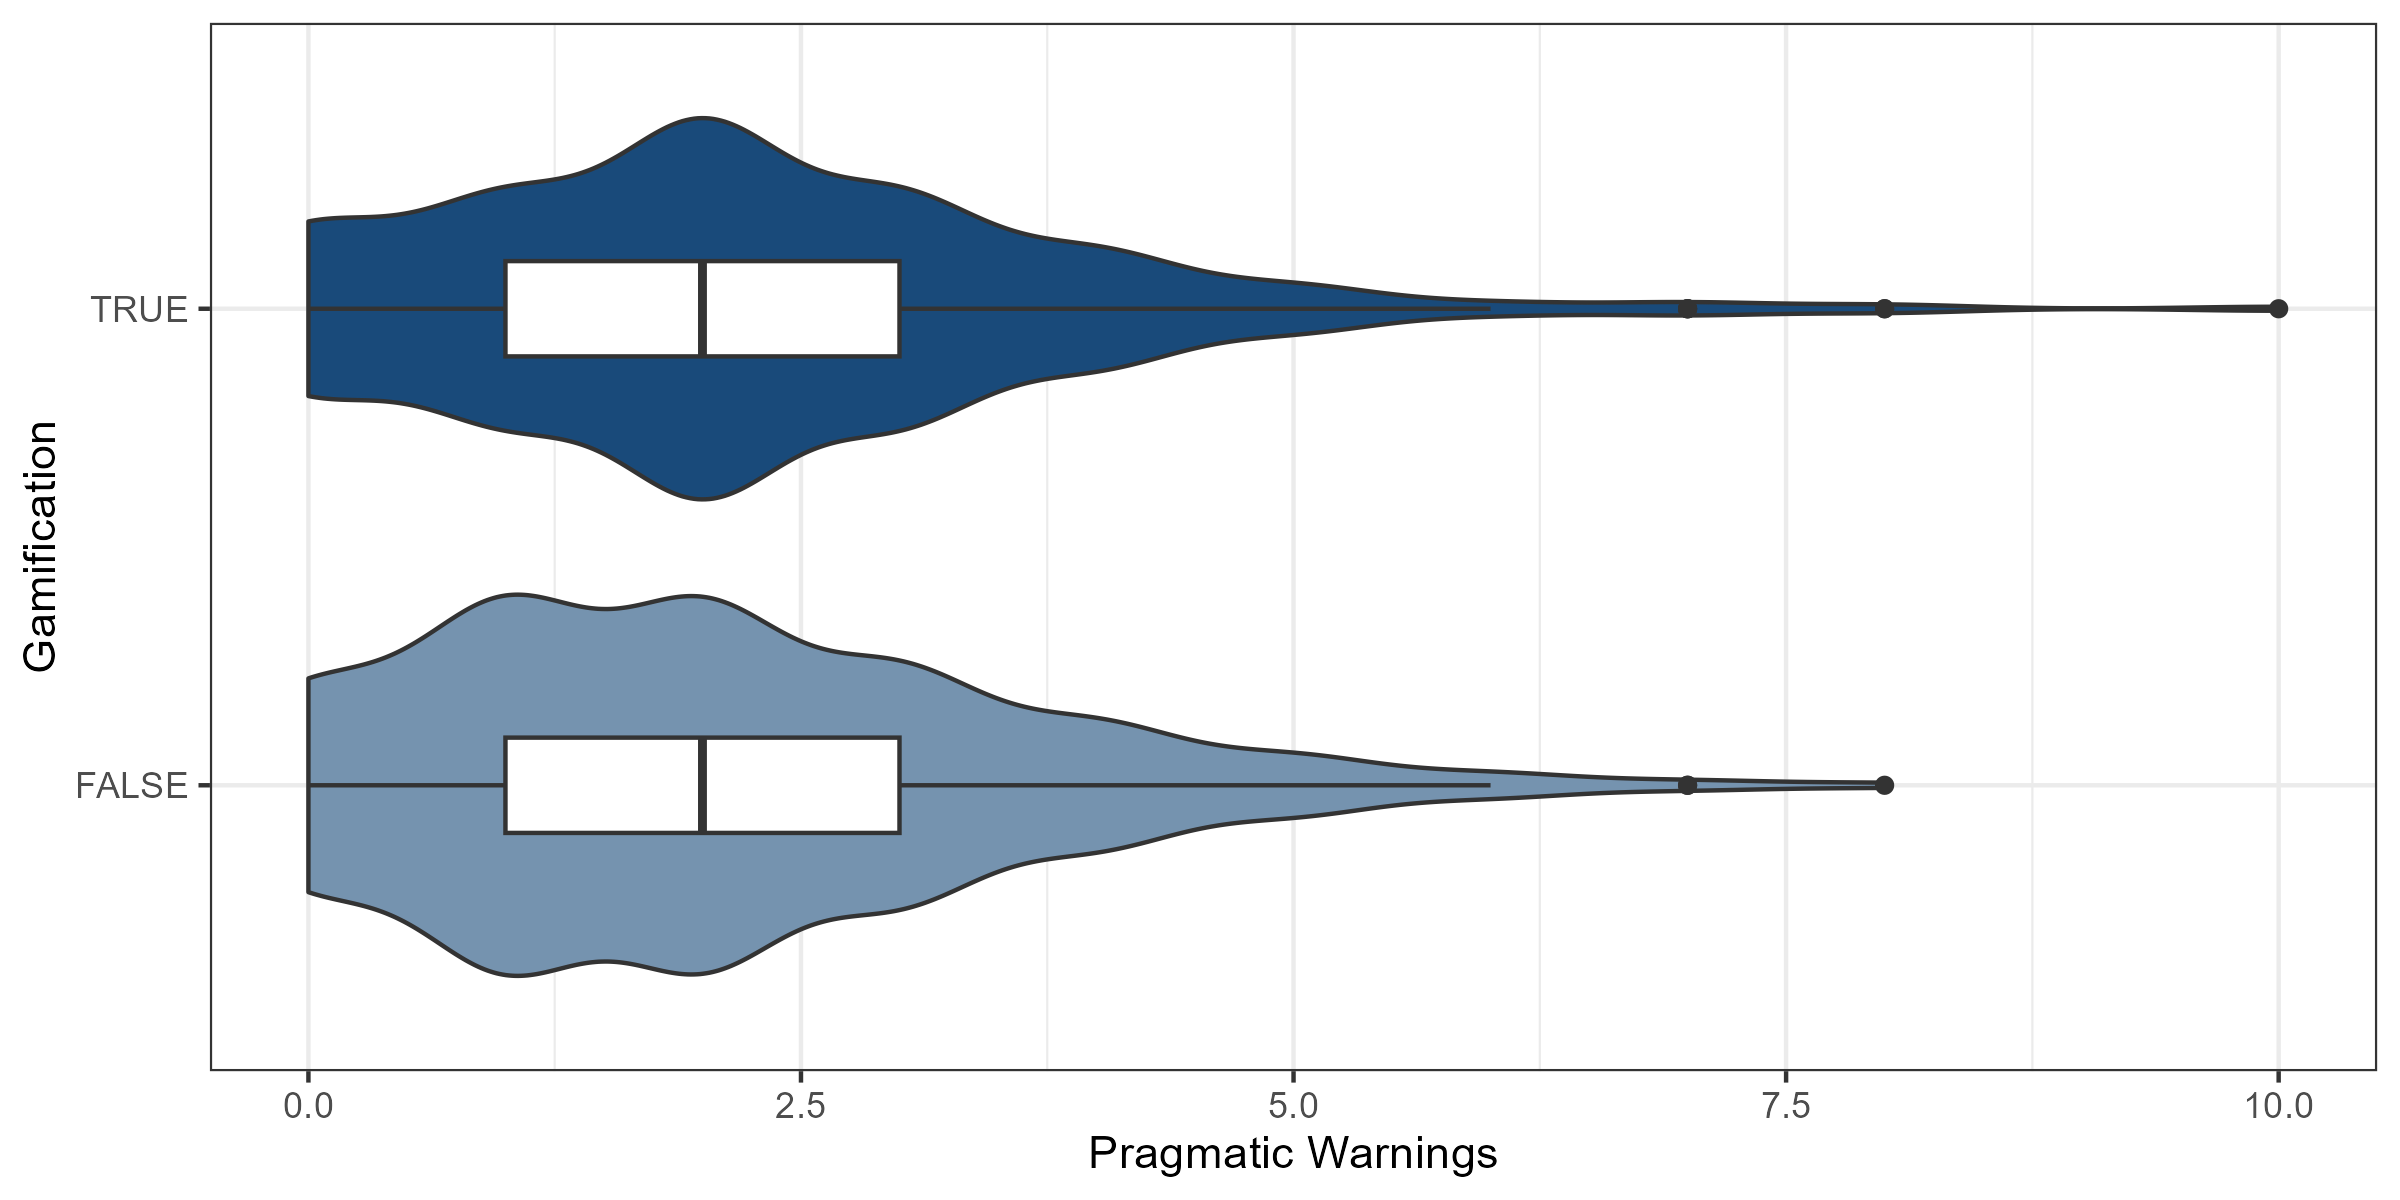
\includegraphics[width=\linewidth]{Template_Latex_ScuDo_Tesi/Chapter4/prag_violin.png}
        \caption{Box and violin plot for the \textit{Pragmatic Warnings} metric}
        \label{fig:rq2_prag}
    \end{subfigure}
    \caption{Box and violin plots for RQ2 metrics}
    \label{fig:rq2_4}
\end{figure}

Overall, the distribution of metrics paints an encouraging picture for what concerns the effect of gamification: diagram completeness is on average higher, and both syntactic and semantic errors are lower as well; it can be assumed that gamification can lead to better student performance, with more correct elements being represented and fewer errors being made. Pragmatic warnings, however, are higher on average when gamification is applied: a possible interpretation could be that, since they are presented as minor issues that do not impact correctness and can simply be represented in a better way, students may have decided to ignore them.

To identify whether the treatment or other design factors could have impacted the correctness metrics an ANOVA test was performed; Table \ref{tab:rq2_4_anova} summarizes the result of this analysis by showing the resulting difference coefficient and corresponding p-value for each of the four metrics and associated null hypothesis for treatment, exercise, and group assignment.

\begin{table}[ht]
  \rowcolors{2}{gray!25}{white}
\footnotesize
\centering
\begin{tabular}{lcccccccc}
    \toprule
    Factor / vars: &
    \multicolumn{2}{c}{${H_{pr_{0}}}$} &
    \multicolumn{2}{c}{${H_{syn_{0}}}$} &
    \multicolumn{2}{c}{${H_{sem_{0}}}$} &
    \multicolumn{2}{c}{${H_{prag_{0}}}$} \\
    & coeff. & p-value & coeff. & p-value & coeff. & p-value & coeff. & p-value \\
    \midrule
    Treatment & 4.6750 & \textbf{2.96e-05} & -1.6107 & \textbf{1.62e-03} & -0.9286 & \textbf{9.80e-05} & 0.1500 & 0.259 \\
    Exercise  & 10.1893 & \textbf{$<$ 2e-16} & -2.3821 & \textbf{2.76e-06} & -3.4143 & \textbf{$<$ 2e-16} & -0.80714 & \textbf{6.82e-10} \\
    Group     & -0.8407 & 0.095 & -0.2993 & 0.192 & -0.0900 & 0.402 & 0.0300 & 0.614 \\
    \bottomrule
\end{tabular}
\caption{Results of the statistical analysis for RQ2 metrics. Statistically significant p-values are in bold ($\alpha = 0.0083$)}
\label{tab:rq2_4_anova}
\end{table}

The ANOVA test shows that, when accounting for the treatment, gamification leads to higher completeness on average with a statistically significant p-value: as a consequence, the null hypothesis ${H_{pr_{0}}}$ can be rejected, and it can be said that gamification leads to more correct diagrams. Similarly encouraging results can be observed for syntax and semantic errors: both metrics yield a lower average count for the gamified version and their corresponding ANOVA tests both obtained a statistically significant p-value, implying that using gamification leads to less errors, on average. Null hypotheses ${H_{syn_{0}}}$ and ${H_{sem_{0}}}$ can both be rejected: gamification has a positive effect on student performance by reducing both syntax and semantic errors, meaning that it could be useful for learning both modeling rules and domain adherence. The non statistically significant p-value for pragmatic warnings means that it is not possible to reject ${H_{prag_{0}}}$.


The analysis focused around confounding factors showed that, when considering the exercise as reference, all four metrics have statistically significant differences, with the second exercise showing a higher average completeness (around 10\% more) and lower counts for both syntax and semantic error and pragmatic warnings, reinforcing the assumption that the second exercise was easier than the first. While this may have an impact on the overall results, the experiment's design counterbalances the exercise's impact, thanks to having students perform different exercises in different order and with different treatments. The positive effect of the design can also be seen by the p-values obtained when analyzing the values according to the order of tasks and treatments: with no statistically significant differences, it can be said that no learning effects were in place.

\answer{RQ2}{Gamification had a positive effect on the overall diagram correctness, leading to an increase in completeness as well as a reduction in both syntax and semantic errors, resulting in more correct diagrams. It can be said that the various features helped students understand what they needed to represent and which specific details had to be corrected. The two exercises selected as tasks had different results as well, with one appearing to be easier than the other, with a statistically significant difference in both completeness (higher on average) and all three error types (lower on average); the potential impact of this discrepancy was however mitigated by the experiment design.}

To answer RQ3 and its sub-questions, a questionnaire divided into multiple parts was given to students at the end of the study. The part related to RQ3.1 dealt with the general usability of the tool as well as the perception of the gamified experience with questions taken from the TAM and GAMEX questionnaires; the distribution of the students' opinions, computed as the average score for each construct of both questionnaires, are shown in Figures \ref{fig:rq3_4_tam} and \ref{fig:rq3_4_gamex}.

\begin{figure}[H]
    \centering
    \begin{subfigure}{0.5\linewidth}
        \centering
        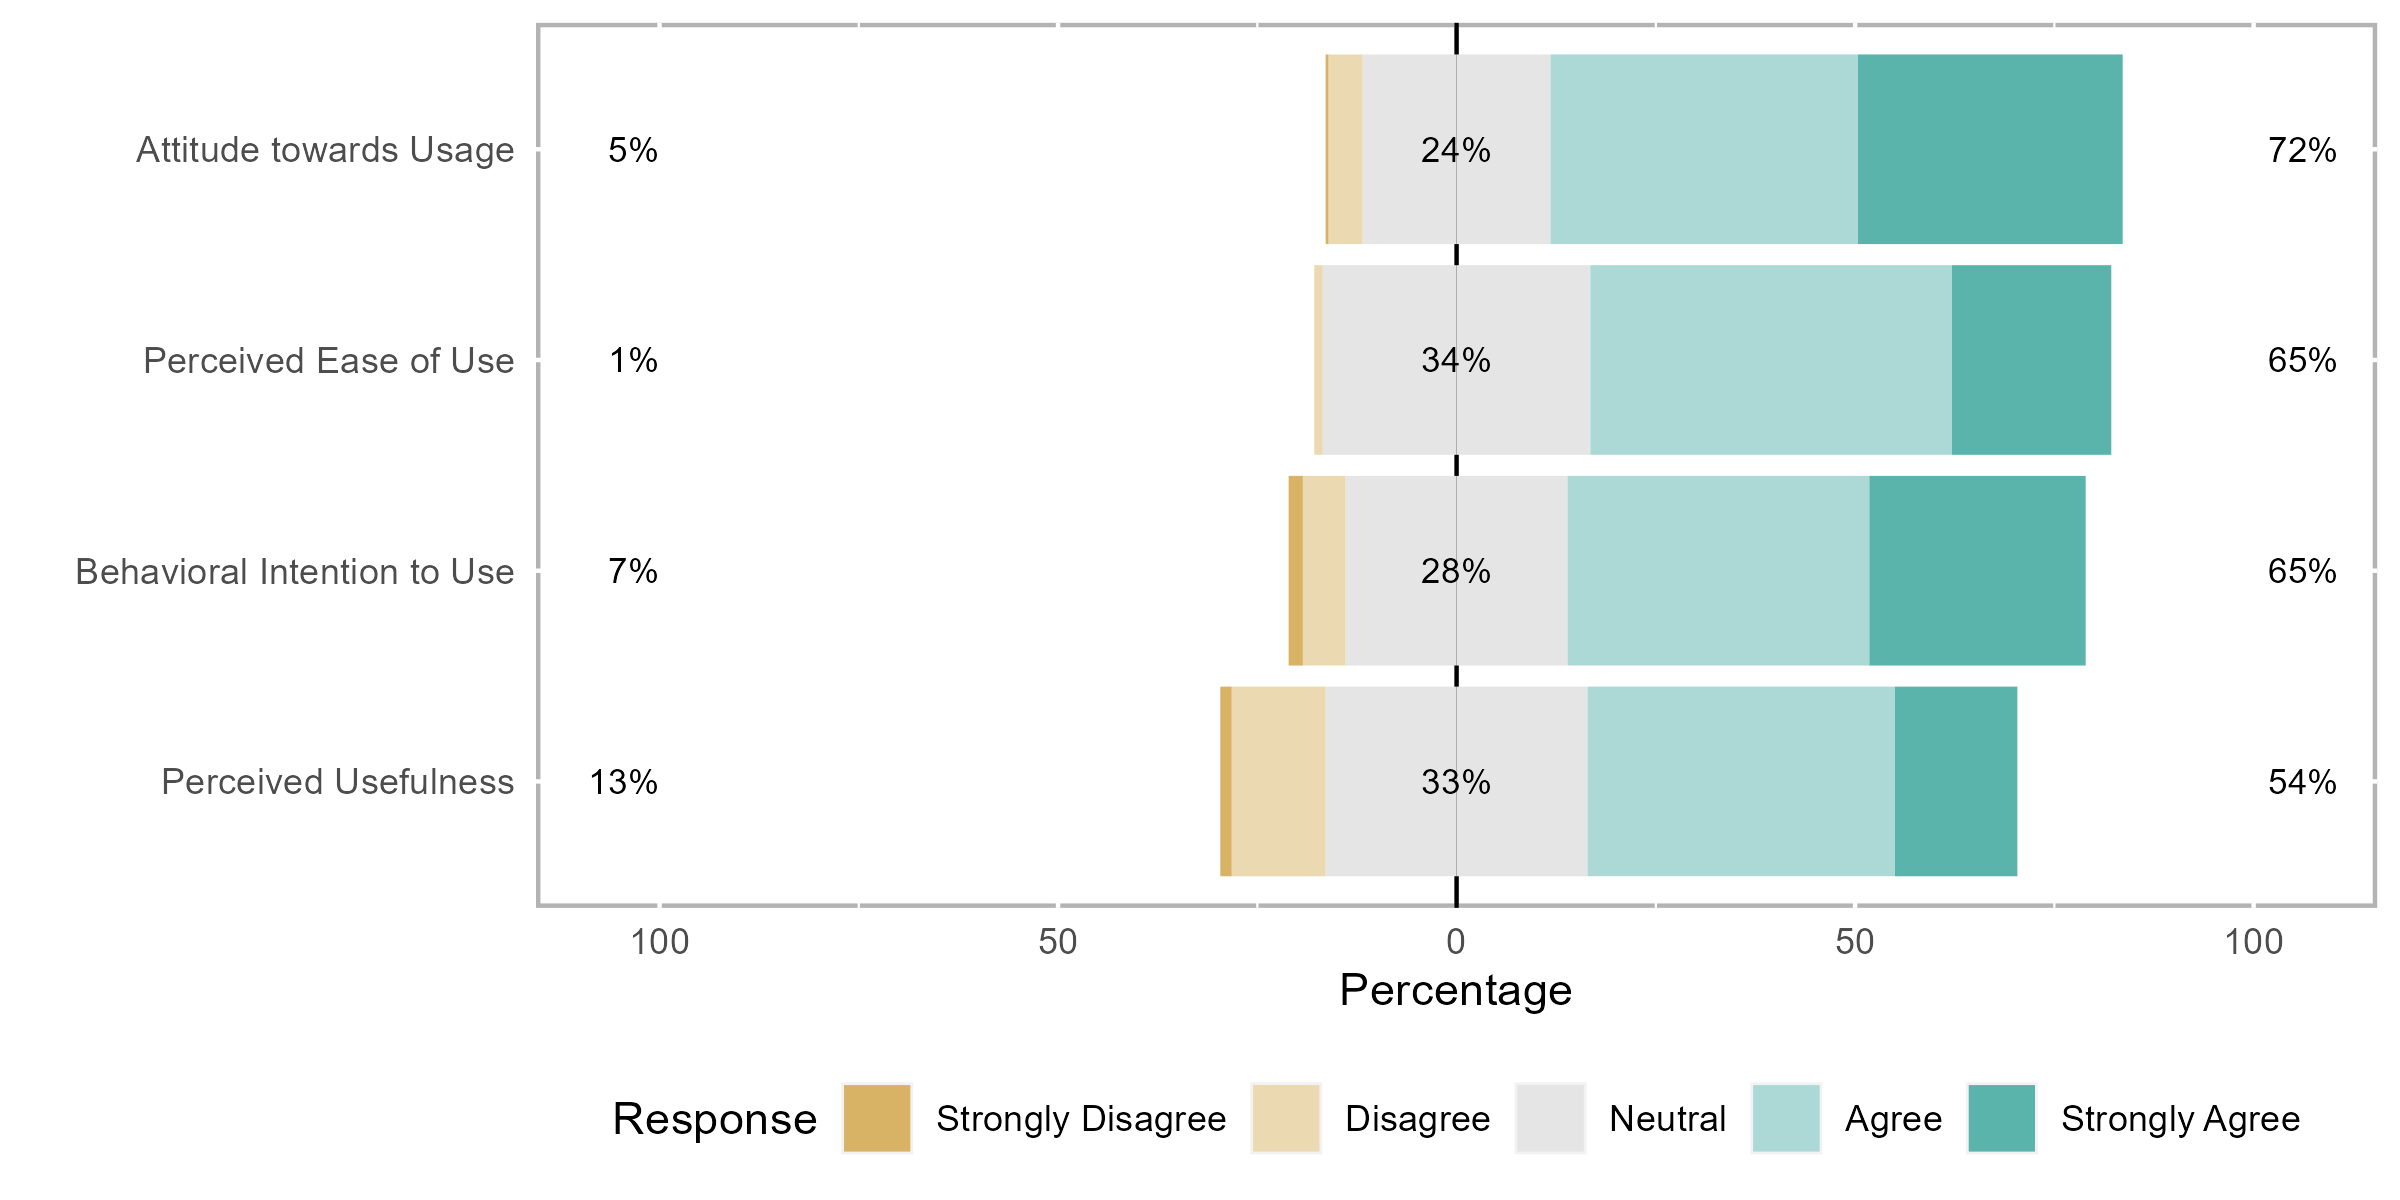
\includegraphics[width=\linewidth]{Template_Latex_ScuDo_Tesi/Chapter4/tam.png}
        \caption{Distribution of answers to the TAM questionnaire}
        \label{fig:rq3_4_tam}
    \end{subfigure}\hfill
    \begin{subfigure}{0.5\linewidth}
        \centering
        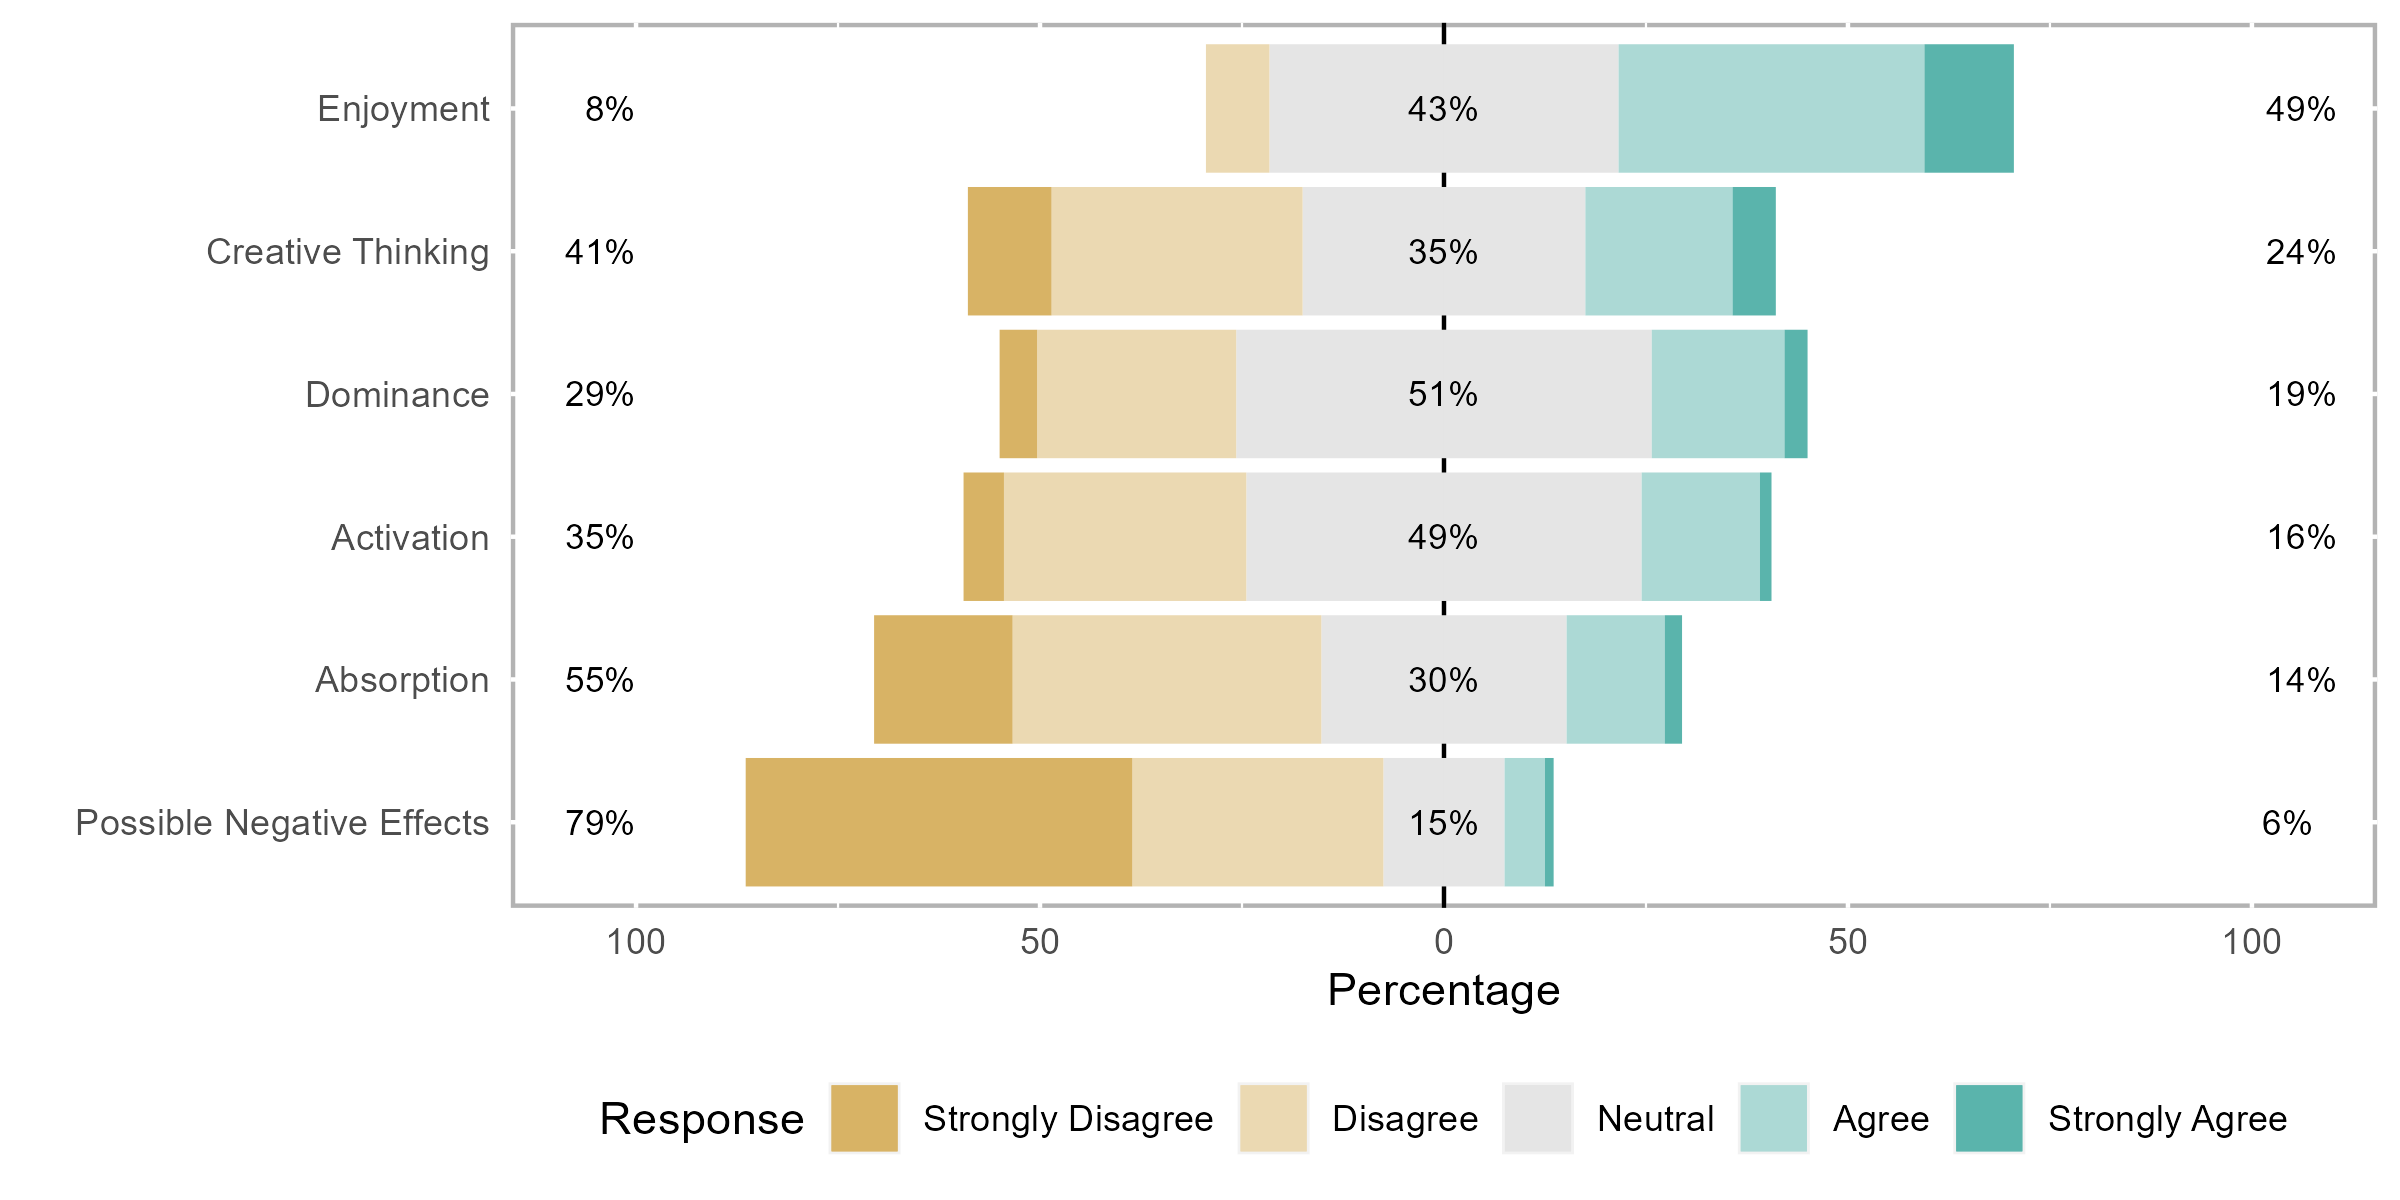
\includegraphics[width=\linewidth]{Template_Latex_ScuDo_Tesi/Chapter4/gamex.png}
        \caption{Distribution of answers to the GAMEX questionnaire}
        \label{fig:rq3_4_gamex}
    \end{subfigure}
    \caption{Distribution of students' average opinions for RQ3.1 constructs}
    \label{fig:rq3_4}
\end{figure}

Regarding answers to the TAM questionnaire, opinions appear to be quite positive, given that at least half of the participants have a positive average opinion (equivalent to answering \textit{Agree} to the entire construct) for each of the four constructs; the distribution of answers given for Attitude towards Usage (72\% Agree + Strongly Agree) and Perceived Ease of Use (65\% Agree + Strongly Agree) are particularly encouraging, since it means that students felt that using UMLegend was something easy to learn, and that it was also a tool students would feel inclined to use more. Negative opinions being quite rare is also a positive result: Perceived Usefulness was the construct with the highest total (13\% Disagree + Strongly Disagree), making it the less successful TAM construct. A possible interpretation could be that the tool appears easy and interesting to use but may not seem as impactful for learning, perhaps as a consequence of using it at the end of a course rather than over time.

Answers given to the GAMEX questions, however, are more on the neutral side, with two thirds of the constructs having a distribution of positive opinions lower than 20\%, with many of them also having at least 30\% total negative opinions. The only clearly positive results obtained with the GAMEX questions concern the Enjoyment construct, with a total of 49\% positive opinions, and the Possible Negative Effects one, with 79\% disagreeing opinions. It can be assumed that UMLegend is perceived as a fun and engaging tool to support modeling activities with very little negative impact such as frustration or hostile design choices.

Unfortunately, since the remaining for constructs tend to have distributions of opinions between neutral and negative, certain limits of the tool emerge: creative thinking is not entirely supported despite the freedom given for modeling choices, and the tool does not feel particularly stimulating and immersive. It is possible that these results depend on the single-session design of the experiment, and that continuous adoption may improve the tool's perception in these aspects.

\answer{RQ3.1}{The UMLegend tool was favorably received by students in terms of its general usability, as highlighted by the answers given to the TAM questionnaire: students felt that the tool was easy to use, and stated they would be inclined to use it for modeling tasks; however, questions related to the perceived usefulness ranked the lowest among all four constructs, meaning that the educational benefits may need to be conveyed more clearly. The gamification-specific perception of the tool, conversely, was not as positive: while most students agreed that using the tool is an engaging and fun experience that does not feel frustrating or makes the player feel antagonized, certain aspects such as the immersiveness or the support for creativity and freedom still feel limited, implying the need for a redesign of certain mechanics.}

The second block of the questionnaire, designed to answer sub-question RQ3.2, included custom made questions repeated for each of the game mechanics that investigated whether students perceived the mechanic as useful, if the mechanic influenced their use of the tool, if students were satisfied with how they interacted with the mechanic, if they felt motivated by it, and if it was perceived as distracting. For each student, the overall opinion was computed similar to how it was done for the TAM and GAMEX questionnaires, given that the answer format was the same (Likert scale values ranging from 1 to 5), although with one difference: since the fifth question had a negative connotation, the average was computed using its opposite value (e.g., a \textit{Strongly Disagree} answer was considered a \textit{Strongly Agree} when computing the value) to offset the negative value. The average answer was computed for each game mechanic, to identify the most appreciated ones; Figure \ref{fig:rq32_4} shows the overall distribution of opinions.

\begin{figure}[htpb]
    \centering
    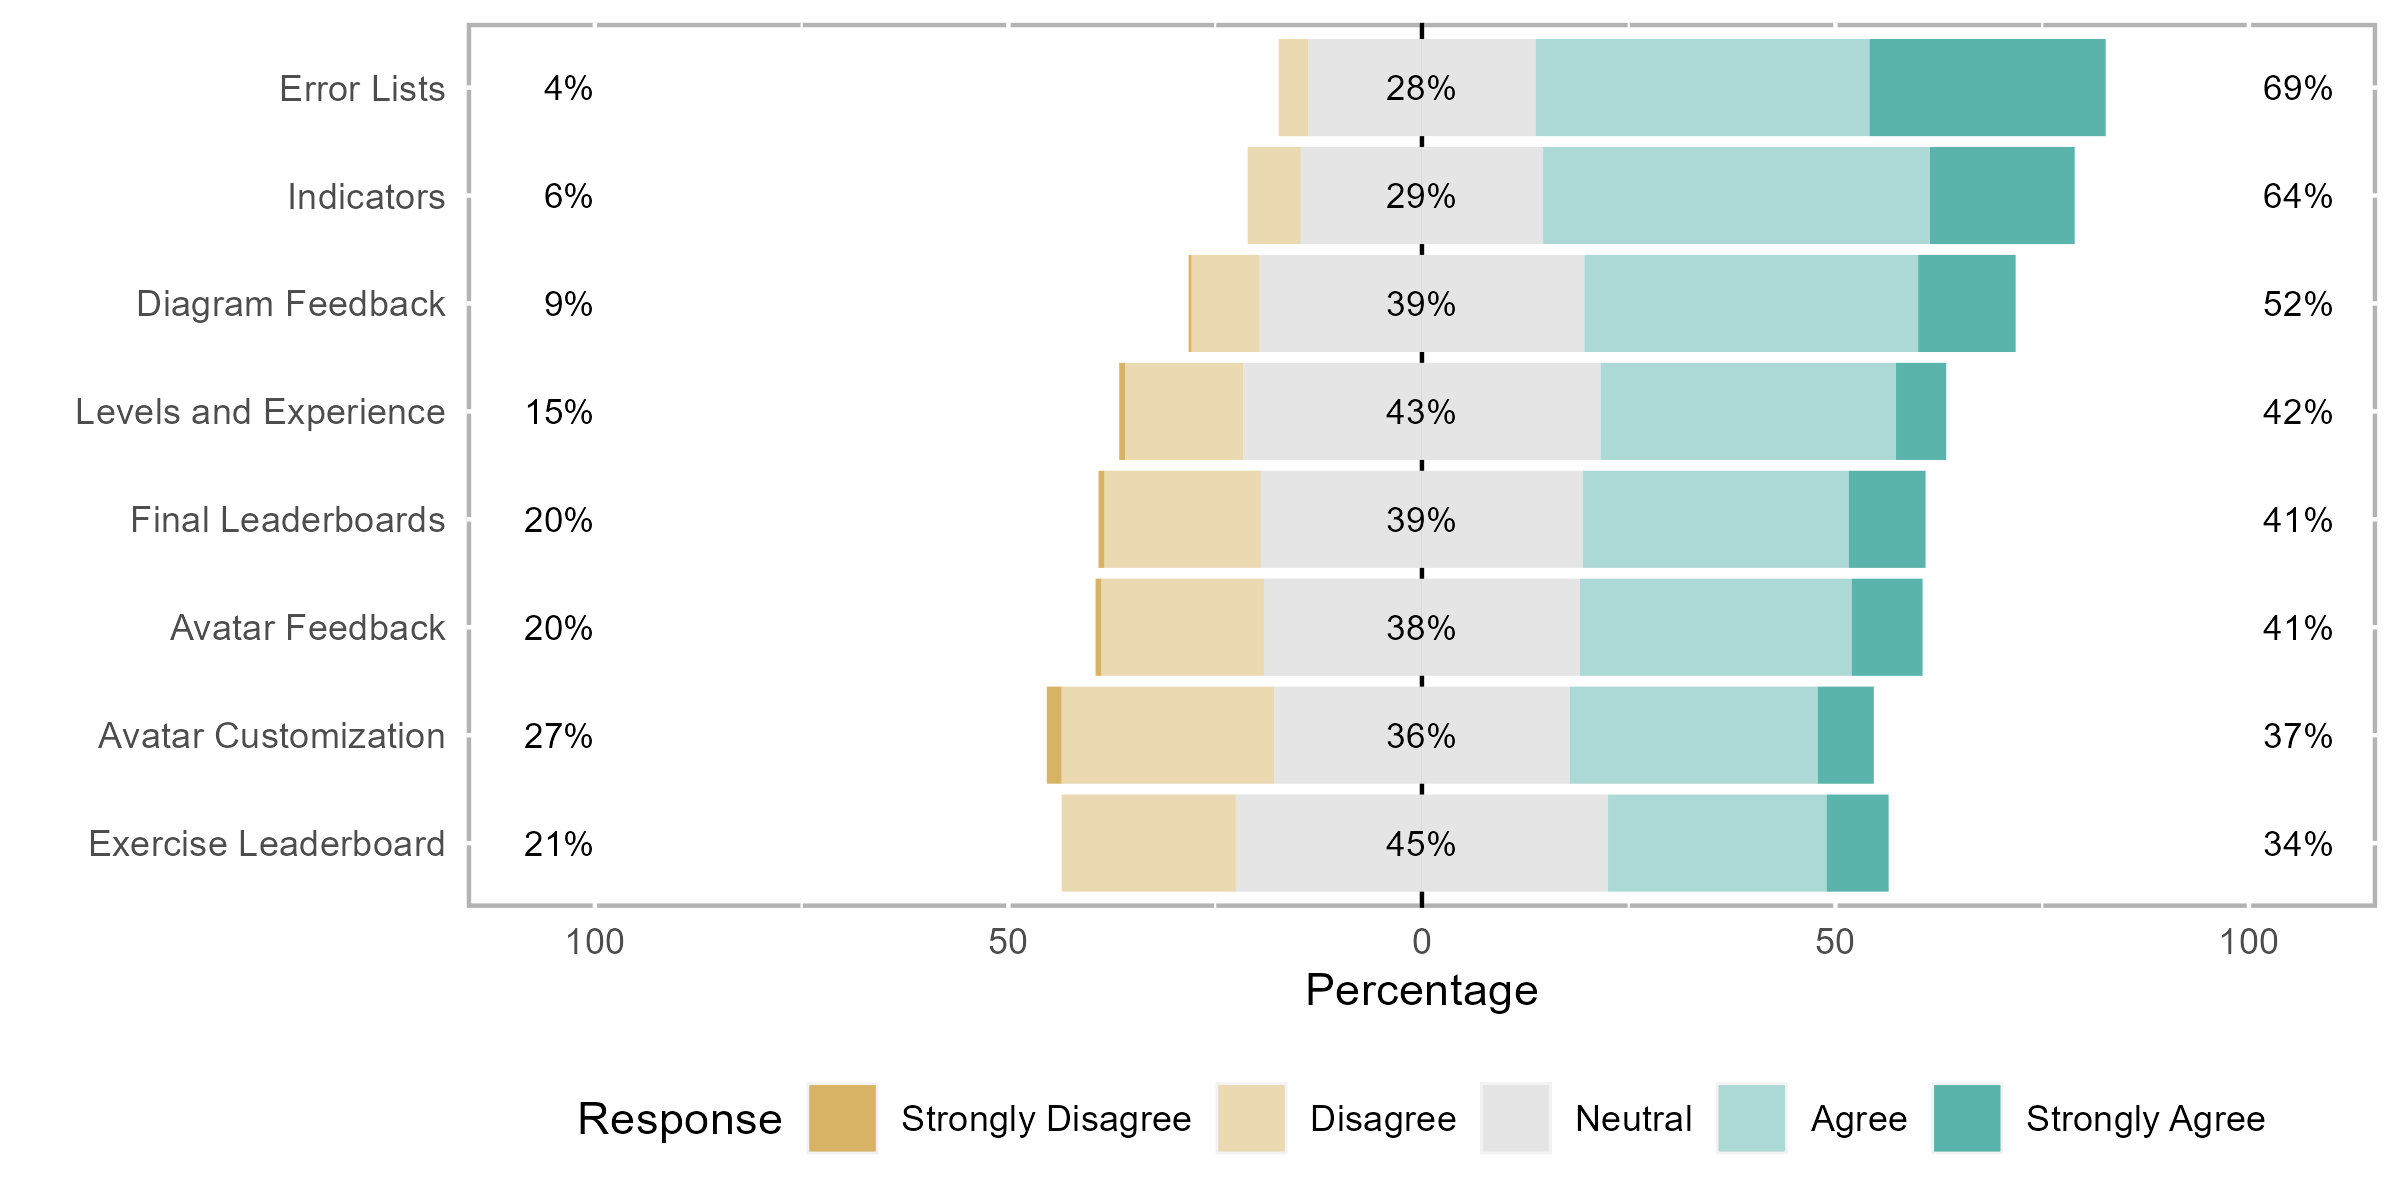
\includegraphics[width=\columnwidth]{Template_Latex_ScuDo_Tesi/Chapter4/mechs.png}
    \caption{Distribution of answers related to the different game mechanics}
    \label{fig:rq32_4}
\end{figure}

Overall, it can be said that all game mechanics have been somewhat well received, with all of them having a positive average opinion of least 33\%. Moreover, the distribution seems to confirm the same perception of game mechanics that was found with the BIPMIN study: game mechanics that provide direct assistance in solving an exercise are the most appreciated, given that for Error Lists, Indicators, and Diagram Feedback at least half of the participants had positive opinions and less than 10\% had negative ones. Mechanics that were conceived for long-term usage such as Leaderboards and Avatar Customization were also well-received, supporting their inclusion in the new framework and reinforcing the necessity for a longitudinal study on gamified modeling education. However, the fact that Avatar Customization was the mechanic with the highest percentage of negative opinions (27\%) may not only depend on the single-session design and on the need to unlock additional props but also on the perception itself, which may appear childish and negatively impact the overall tool perception.

\answer{RQ3.2}{All game mechanics have been appreciated by at least a third of the participants, suggesting that the redesign was successful and encouraging future and continuous use of UMLegend. The detailed distribution of opinions confirms what was discovered with the first empirical study: mechanics that provide direct assistance for completing exercises by specifying what needs to be improved and how are the most appreciated, and mechanics intended for long-term usage rank slightly lower.}

Lastly, the final block of the questionnaire consisted of two open-ended questions, one asking for issues encountered when using the tool and another asking for suggestions and possible improvement areas. After performing an open-coding analysis on the answers given by students, a total of 6 topics were found for the first question, after excluding 227 answers that reported no issue; similarly, 142 answers to the second question were either empty or had no suggestion and were not considered for the analysis. The topics found in the two questions can be seen in Figures \ref{fig:rq3_4_issues} and \ref{fig:rq3_4_issues}.

\begin{figure}[H]
    \centering
    \begin{subfigure}{0.5\linewidth}
        \centering
        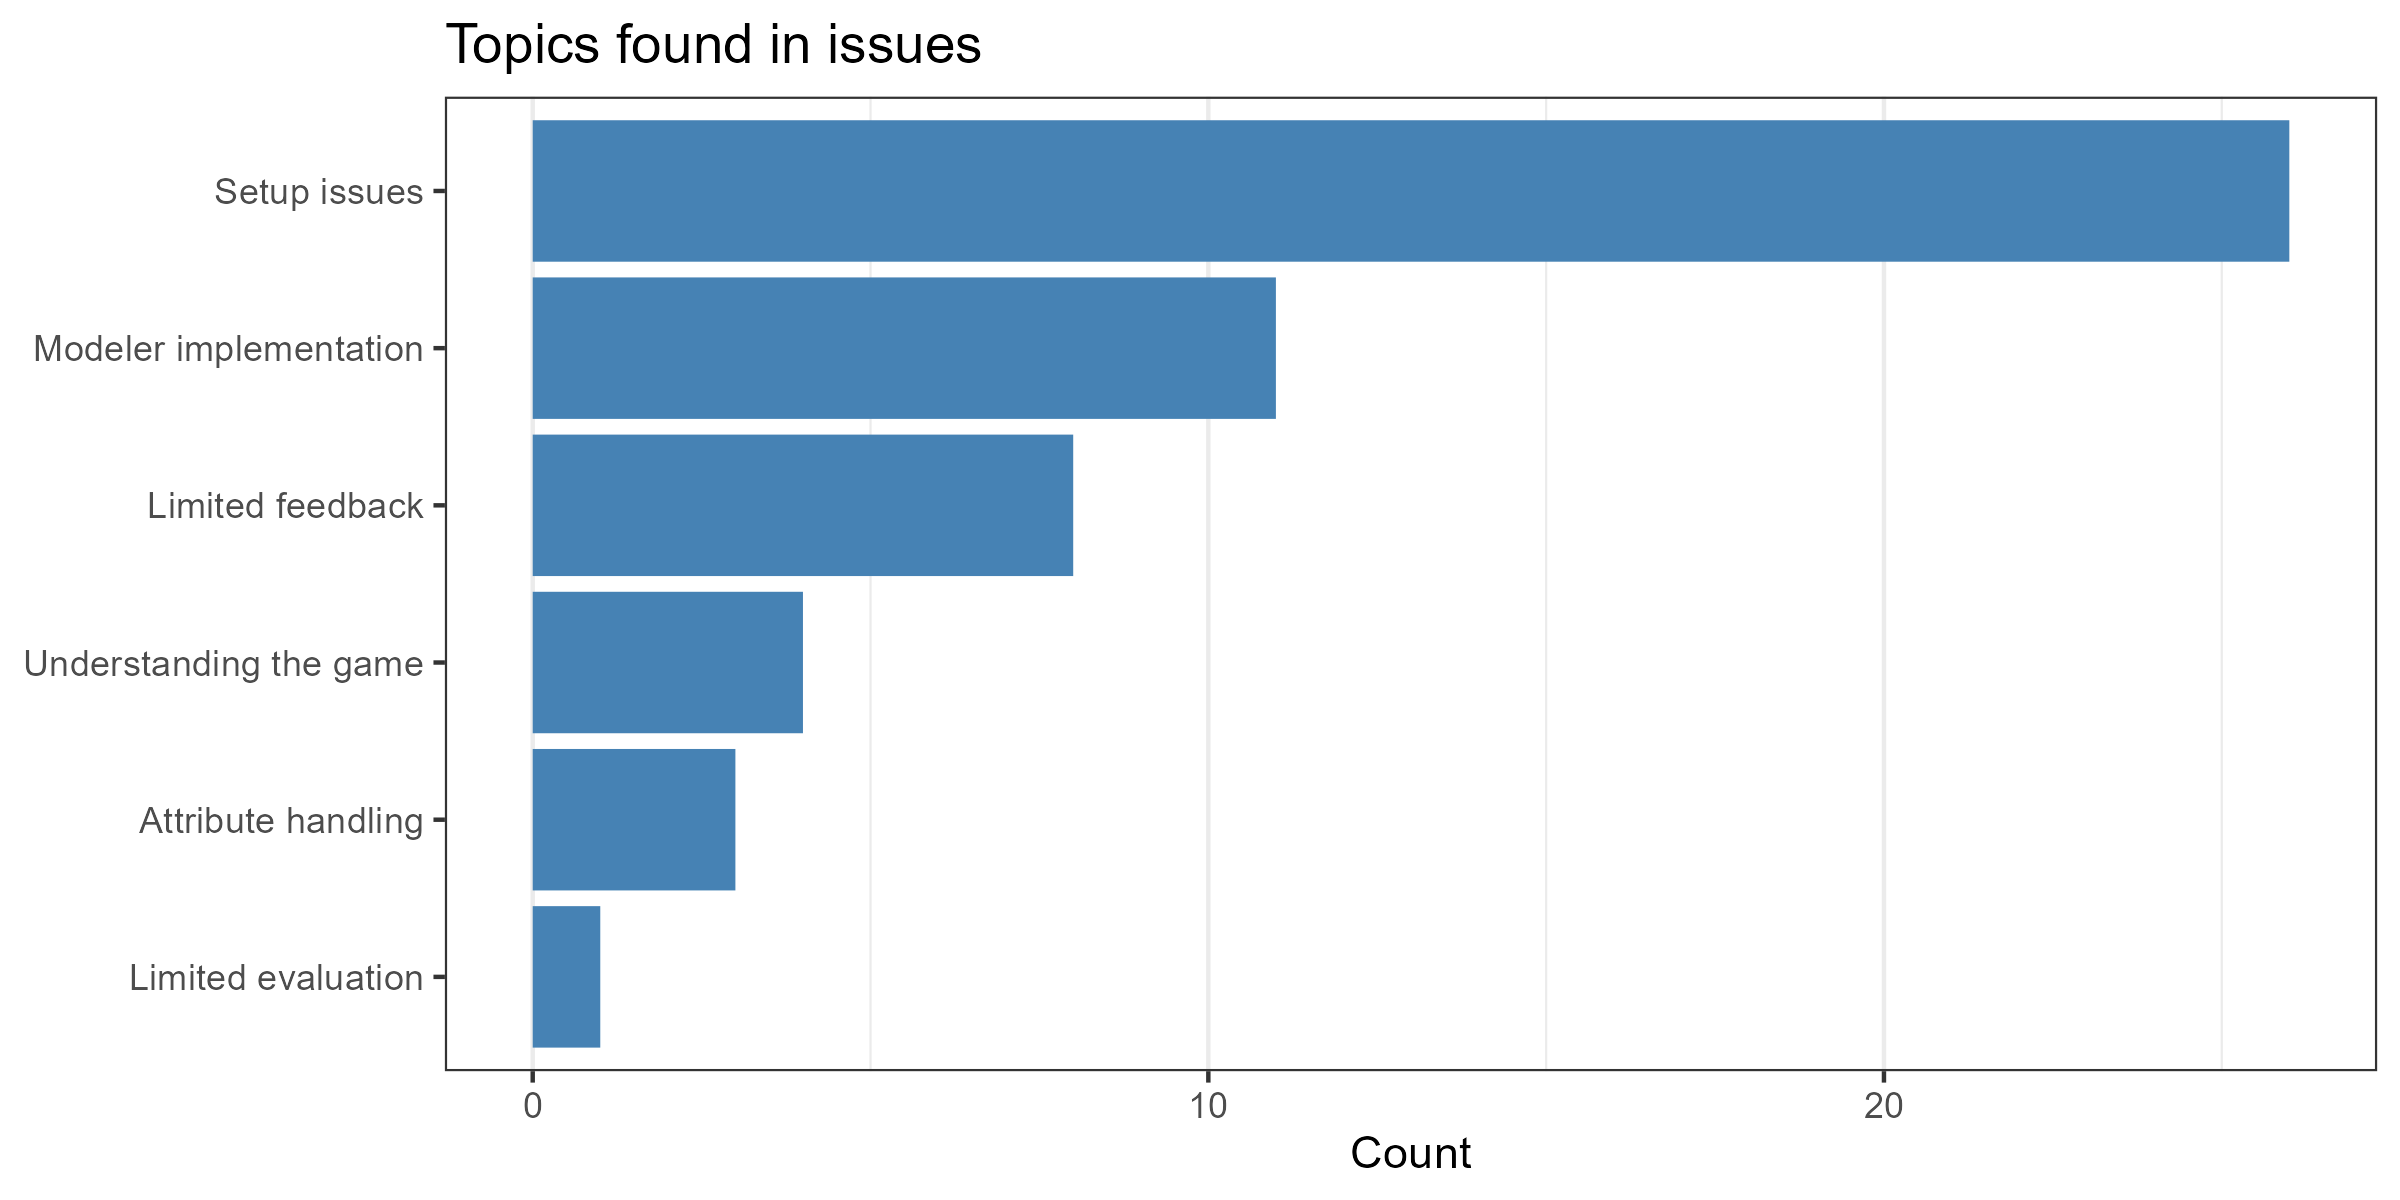
\includegraphics[width=\linewidth]{Template_Latex_ScuDo_Tesi/Chapter4/issues.png}
        \caption{Topics found in the open-ended question asking for issues encountered during the study}
        \label{fig:rq3_4_issues}
    \end{subfigure}\hfill
    \begin{subfigure}{0.5\linewidth}
        \centering
        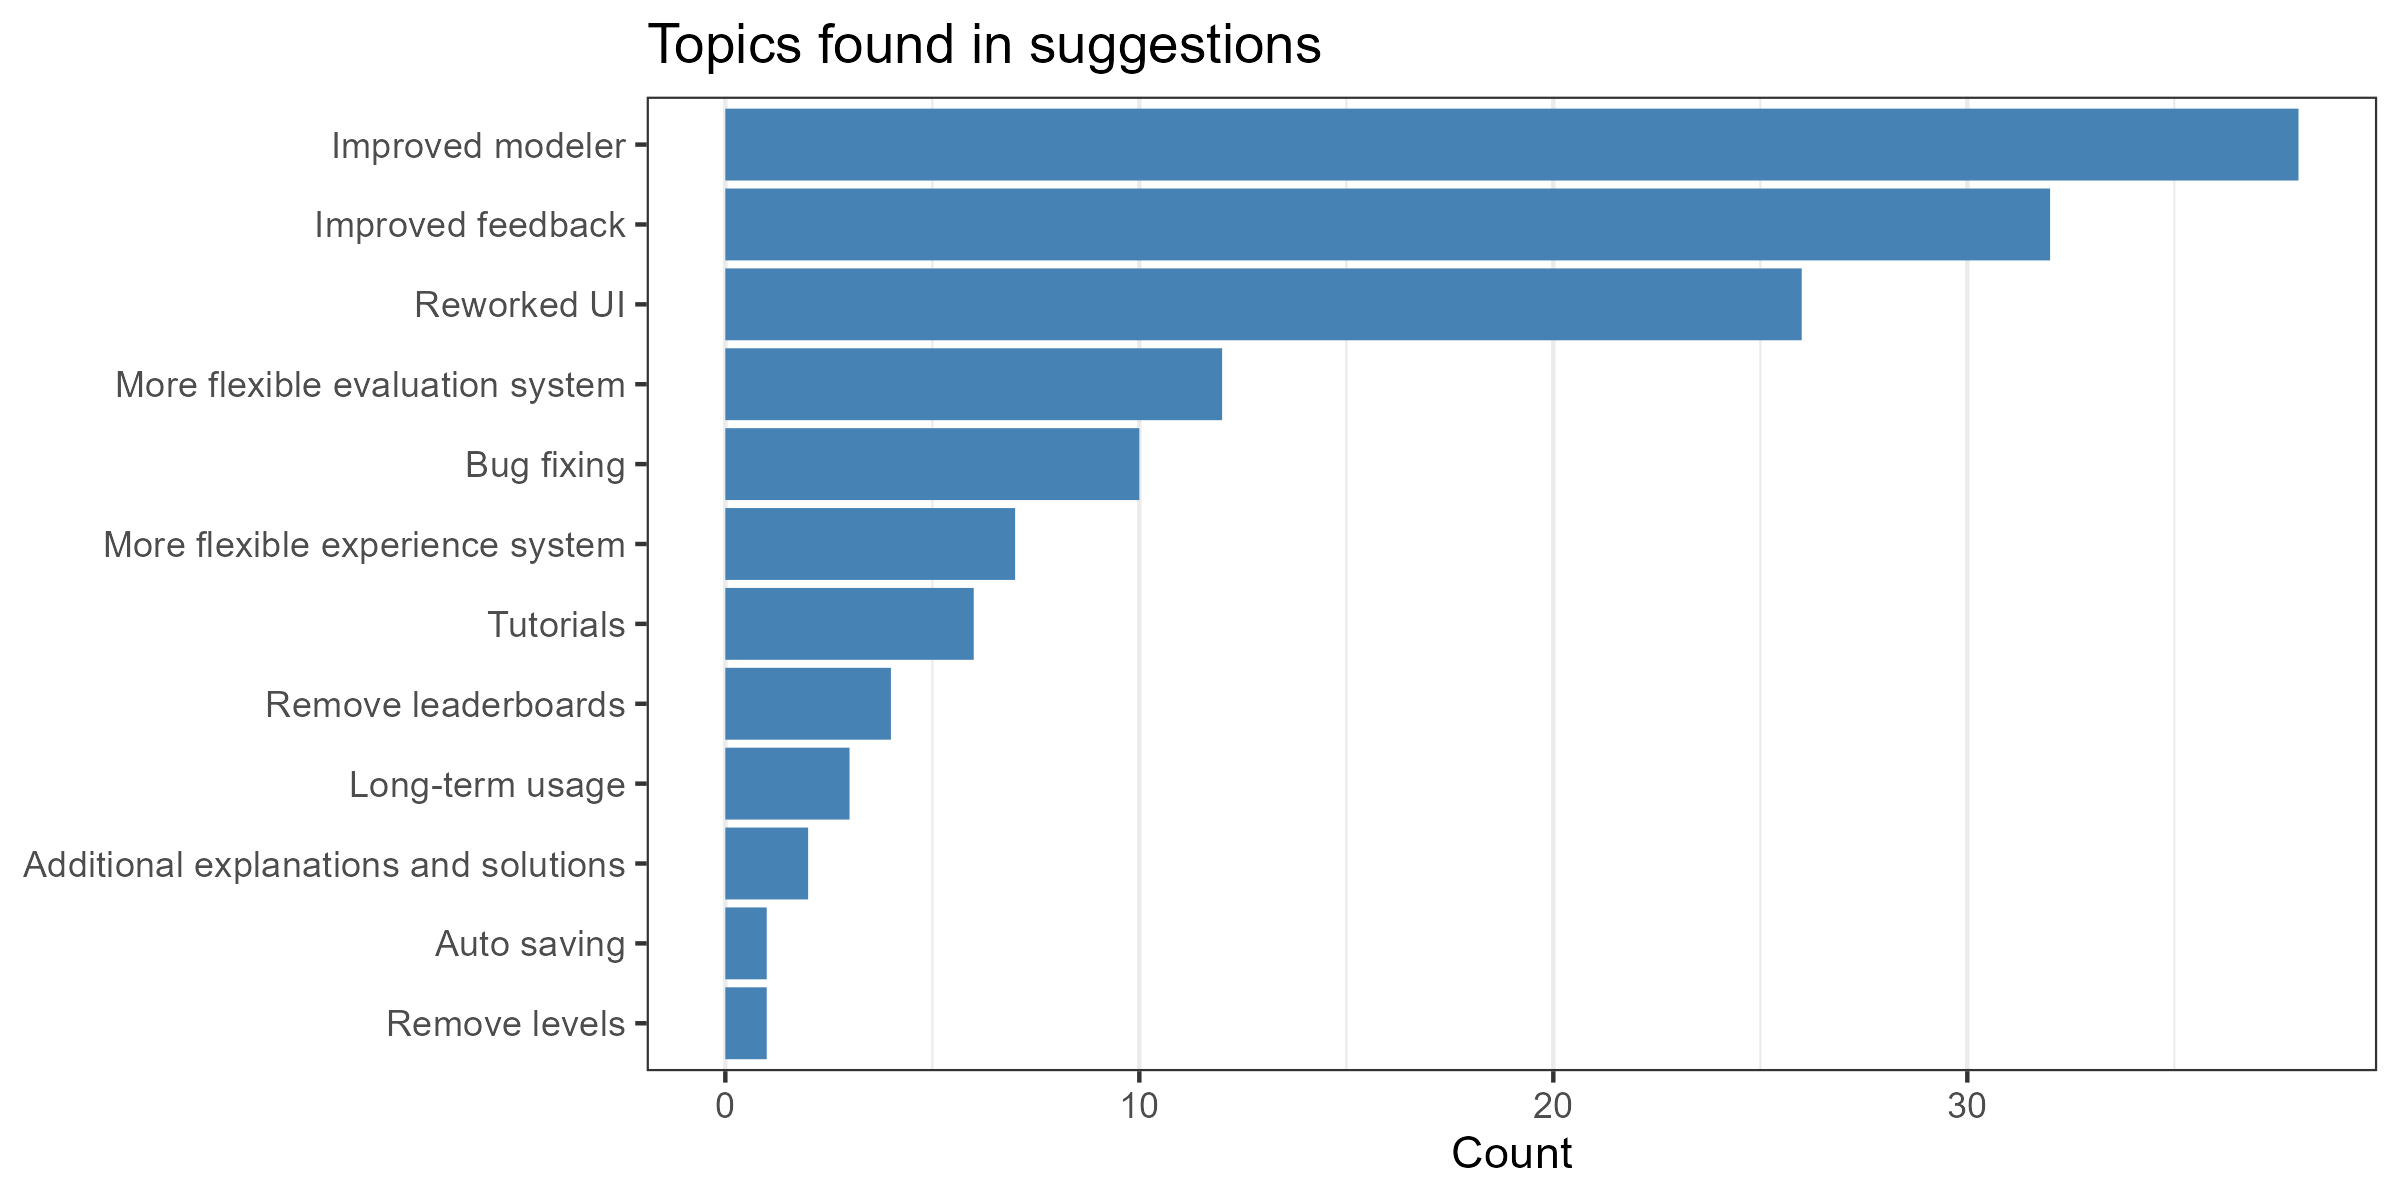
\includegraphics[width=\linewidth]{Template_Latex_ScuDo_Tesi/Chapter4/improv.png}
        \caption{Topics found in the open-ended question asking for suggestions for improving UMLegend}
        \label{fig:rq3_4_impr}
    \end{subfigure}
    \caption{Results of the open coding procedure on the answers given to the two open-ended questions}
    \label{fig:rq33_4}
\end{figure}

Regarding issues, the most common topic related to issues in setting up the tool and using its features, something that depends on the explanations given at the beginning of the study, that may have been unclear or limited; more relevant issues cover problems in the modeler implementation and the feedback, which was judged limited and unclear. The modeler issues may depend on the fact that students were used to a different modeling tool (Signavio Academic), with more features compared to the Apollon modeling library used in the tool such as an easier way to specify attributes or better association handling, a part of the modeling interface that was considered complex and unfriendly.

These two topics found in issues were also found in the answers given to the question asking for suggestions: an improved and friendlier modeler, closer to the one students were used, was the most common request, indicating that perhaps the neutral perception of the tool depended not only on the game mechanics but on the modeling aspect as well. The feedback mechanisms were also mentioned by several answers as something that could be improved by explaining errors more in detail or by also highlighting correct elements.

Other common suggestions mentioned reworking the user interface by changing the way an exercise's text is displayed or letting students select text from the description and create classes starting from the text; certain comments also stated the need to make the evaluation engine more flexible, since there were scenarios in which certain synonyms were not considered valid despite being correct due to not appearing in the reference solution. Experience management was also mentioned as a part of the system to revise, since students stated they did not feel that correcting errors actually helped increase the experience reward again, and errors reducing the value felt more impactful; suggestions to address this issue mentioned either reducing the penalty caused by erorrs or having errors reduce experience only on their first appearance.

Lastly, rarer suggestions covered once more findings from the original BIPMIN study related to the single-session design: leaderboards and levels were not considered impactful, with some students suggesting their removal, tutorials were also mentioned as a potentially relevant feature, and some students explicitly stated they would have preferred using the tool more if it was available for a longer period of time.

\answer{RQ3.3}{The analysis of the students' open comments helped identify certain limitations of UMLegend such as the somewhat unfriendly modeling interface, the need to expand feedback to be more detailed, potential improvements to the user interface, and a rework of the experience management to make it more friendly and less penalizing. The evaluation engine was still a point of concern due to issues with certain synonyms and modeling choices not being considered in advance for the reference solution, but was a less severe problem in comparison with the 2023 study.}

\subsection{Threats to validity}

Following the characterization by Wohlin et al. \cite{wohlin2012experimentation}, the threats to the validity of the empirical study are discussed below.

\textbf{Threats to internal validity:} the crossover design could have introduced learning effects, due to having students perform two tasks consecutively and using tools with a common base; it may also be possible that the second task may have been influenced by the first one. The different difficulty level of the two exercises, which emerged during the analysis, may also have impacted the results. The choice to use a 2x2 factorial design mitigated these threats. 

Other relevant internal threats depend on the limited variability in the reference solution, since certain correct modeling choices may not have been recognized as such, potentially introducing a negative bias in the evaluation of the diagrams. The use of synonyms for each named elements and the support for small grammar mistakes and typos mitigated this threat.

Lastly, considering feedback a game mechanic may also have had an impact on the results: using a detailed feedback mechanism in the gamified version and a simplified, generic one for the non-gamified one may have reduced the scores for the latter version.

\textbf{Threats to External Validity:} it may not be possible to generalize the results to students with different modeling skill levels. For example, performing a similar study at the beginning of the course may yield different results, same performing it with students from a different background. Moreover, the benefits may apply specifically in an university setting and not in industrial modeling scenarios.


\textbf{Threats to Construct Validity:} the metrics observed to answer the research questions may not be the most suitable to represent the actual observed constructs. For example, productivity may have been measured with the time spent to complete each exercise, although such metric does not necessarily imply better performance, and correctness may have been measured with different rules and criteria, perhaps yielding different completeness scores and error counts.


\textbf{Threats to Conclusion Validity:} non-parametric statistical tests were used, and since all metrics were collected automatically by the tool the risk of human errors was minimized. There may have been a risk of confounding factors depending on the random allocation of participants to the four groups, resulting in certain groups having more capable participants, but this threat can be considered improbable with the assumption that participants all had a similar modeling skill level due to performing the study at the end of the course.

\subsection{Key findings and lessons learned}

The empirical study aimed to continue what was started with the 2023 study by investigating whether a gamified modeling tool, developed according to the lessons learned from the first study, could have a positive influence on student performance and be well received by a sample of the intended users for such a tool (university students of modeling courses). The results were more encouraging compared to the first study, and helped identify key issues to address in the latter part of the PhD course. 

A relevant result comes from the positive impact of gamification on the number of evaluated checks made by students: while this confirms a similar trend identified in the first empirical study, it also strengthens the conviction that modeling activities benefit from game mechanics being tied to automated diagram assessment and auto-evaluation, leading to an increase in student commitment.

Additionally, gamification also had a positive effect on diagram correctness, with both higher average completeness and lower average syntax and semantic error counts. This result is particularly encouraging when compared to the original study's result, where only semantic correctness was positively affected by gamification; moreover, the original interpretation of semantic correctness for the 2023 study could be considered equivalent to the overall diagram completeness, rather than the adherence itself to the intended domain. As a consequence, the UMLegend study confirmed the benefits of gamification on helping students represent correct diagrams, and also introduced the possibility of said strategy being useful for learning modeling rules. 

The revised implementation of game mechanics also led to an improvement in student perception: the post-study questionnaire showed that UMLegend is a fairly easy to use application, with potential for long-term use and possible benefits, while also being fun, engaging, and with little to no negative aspects such as frustration or hostility toward users, according to the students; certain gamification-specific aspects, however, were not all rated as highly, with limited freedom of action and creativity, as well as immersiveness, being causes of concern. These observations are also in line with the original study, and point to a limitation in the single-session experiment design: it may be reasonable to assume that longitudinal usage would increase aspects such as freedom and immersion.

The post-study questionnaire also confirmed the findings described in Chapter 3 related to game mechanics: students tend to appreciate the most mechanics such as diagram feedback or error lists that directly point out what are the errors in a diagram and provide explanations on how to correct them, while mechanics intended for longitudinal use such as levels and leaderboards, while still appreciated, were considered less impactful, with a few students even suggesting their removal from the tool. It can be deducted that single-session studies, while effective for understanding whether gamification can improve diagram completeness and student understanding of modeling rules, are not sufficient to properly assess the benefits and perception of gamified modeling education, and longitudinal studies are also necessary.

Lastly, while results are overall positive and encouraging, certain issues remain such as the unfriendly modeling canvas, which felt frustrating to use compared to the platform students were used to, the excessively strict experience system, which was considered too penalizing, although with less frequency compared to similar complaints recorded after the first study. The evaluation engine was also mentioned by students as a limit of the tool, despite the implementation allowing for more synonyms and variations in names, certain correct modeling choices were marked as incorrect; this was the most common issue in the original study, and it still appears to be a relevant problem to consider, although far less students mentioned it as such.

\articleSummary{
color1
}{
Summary of the empirical study
}{
The empirical experiment demonstrated that the new gamification framework can positively affect student commitment, diagram correctness and student understanding of modeling rules, with higher diagram completeness and fewer syntactic and semantic errors. The students' reception of the tool's usability was largely positive, while the gamified experience was perceived as enjoyable but not fully immersive, an expected limitation given the single-session nature of the study. The feedback mechanics were the most appreciated components of the tool, reinforcing the design priority given to immediate, actionable feedback in the framework. The main areas for improvement concern the modeling interface, whose perceived unfriendliness detracted from the overall experience, and the evaluation engine, which would benefit from greater flexibility in accepting alternative correct solutions.
}
\begin{comment}
    
\subsubsection{Limitations}
\label{sec:eval_limitations}

Two design limitations of the current evaluation engine are worth stating explicitly, as they directly informed the research directions outlined in Section~\ref{sec:future_work}.

\emph{Single reference solution.}  The engine compares the student diagram against exactly one canonical solution.  An alternative representation that a human evaluator would accept as correct—for example, modelling a concept as an intermediate class rather than as a plain association—may be flagged as an error if the reference does not include it.  Synonym lists mitigate this issue for naming variation but cannot address structural variation.

\emph{Synonym completeness.}  The quality of the semantic matching depends on the exhaustiveness of the synonym lists defined by the instructor.  A valid student label that was not anticipated during solution creation will be classified as non-matching, producing a false-negative.  The open-ended questionnaire responses collected in the experiment (Section~\ref{sec:results_rq3_3}) confirm that this limitation was noticeable to students: improving the modeller was the most frequently cited topic (38 answers), while a more flexible evaluation system was the fourth most common (approximately 20 answers).

Both limitations motivate the use of large language models as semantic similarity judges, an avenue that is explored as part of the future research programme described in Chapter~\ref{ch:future}.

\end{comment}